\chapter{Risultati}
In questo capitolo viene dimostrato il funzionamento dell'applicazione su un Samsung s9 e un Iphone 13, in modo da visualizzare le piccole
differenze di funzionamento e grafica sui due dispositivi.
\section{Splash Screen}
Ogni volta che l'utente apre l'applicazione viene presentato lo Splash Screen mostrato nelle Fig 4.1 e 4.2 . Osservando attentamente le due figure non si notano differenze significative, se non che la dimensione del testo nell'iPhone 13 \`e notevolmente pi\`u piccola.
Inoltre, nel dispositivo Apple il testo \`e posto pi\`u in basso nello schermo: ci\`o \`e  dovuto ad una dimensione maggiore del dispotivo fisico.

Cliccando sul pulsante ``Explore" l'utente potrebbe essere reindirizzato su due screen alternativi: ``Sign in" o ``Images Cache" .\\ \\ \\
\begin{figure}[h]
    \begin{minipage}[h]{0.47\textwidth}
        \centering
        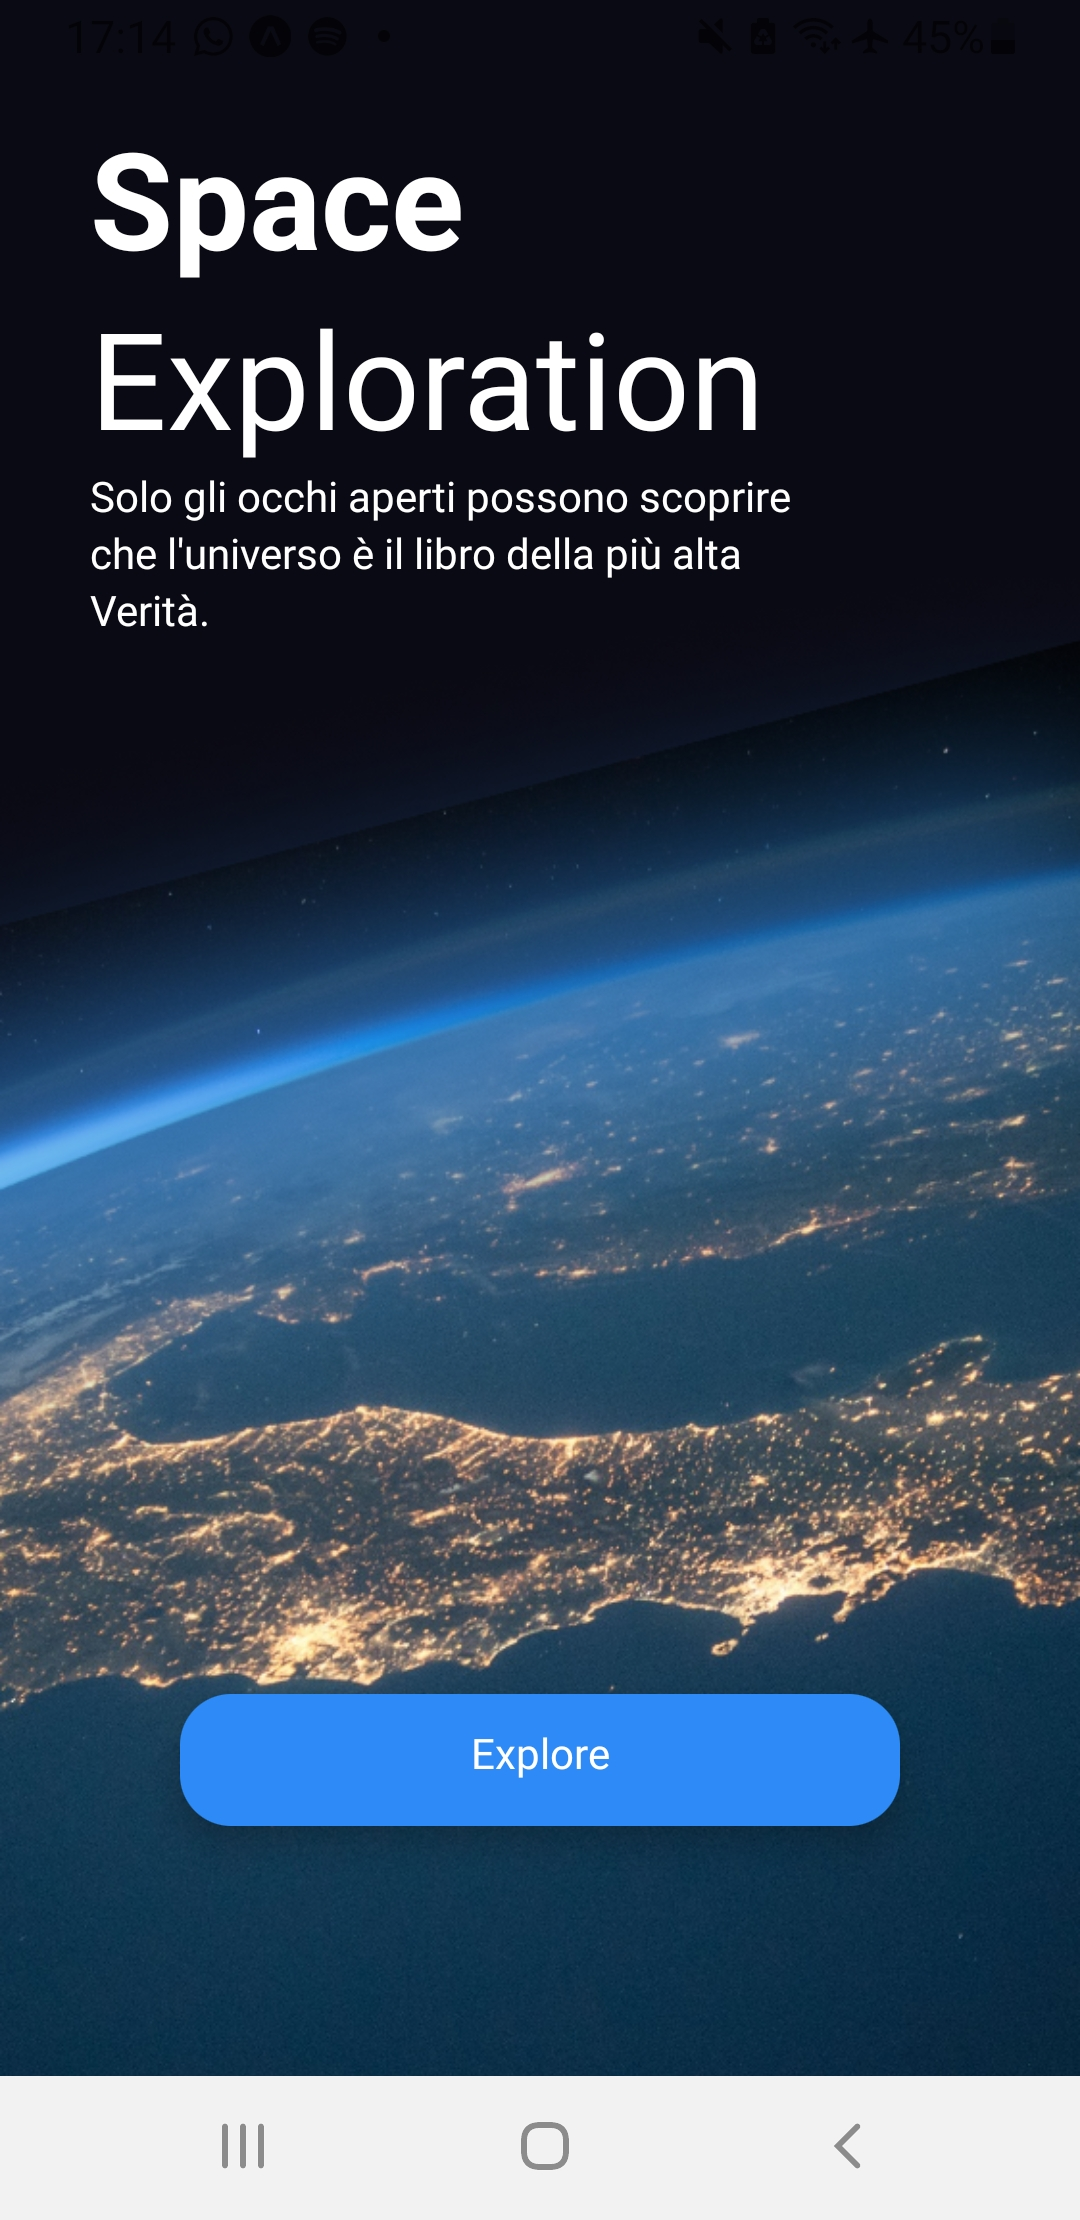
\includegraphics[width=5cm, height=10cm]{images/immaginiAndroid/splashScreen.jpg}
        \caption{\label{SpalshScreenAndroid} Android Splash Screen}
    \end{minipage}
    \hfill
    \begin{minipage}[h]{0.47\textwidth}
        \centering
        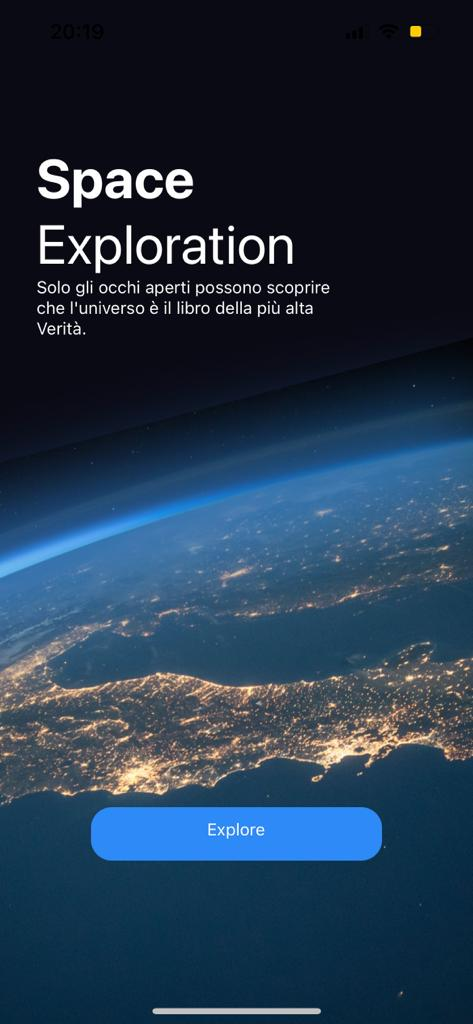
\includegraphics[width=5cm, height=10cm]{images/immaginiPhone/splashScreen.jpeg}
        \caption{\label{splashScreenIphone}iPhone Splash Screen}
    \end{minipage}
\end{figure}


\section{Sign In e Sign Up}
Se l'utente non ha mai effettuato l'accesso all'applicazione, dallo splash screen viene reindirizzato allo schermo di ``Sign in", mostrato nella Fig 4.3 (4.4 per iOS), dove pu\`o accedere al suo profilo con le proprie credenziali.
Nel caso in cui l'utente non abbia gi\`a un profilo , cliccando sul pulsante ``Sign up" viene portato nella schermata di registrazione mostrata nella Fig
4.5 (4.6 per iOS); in quest'ultima inserendo la propria e-mail e password pu\`o registrarsi ed accedere alla schermata principale.
Nel caso in cui l'utente cerchi di accedere con delle credenziali non valide oppure voglia registrarsi con una e-mail gi\`a
presente nel database, viene presentato un messaggio di errore.
\begin{figure}[H]
    \begin{minipage}[h]{0.47\textwidth}
        \centering
        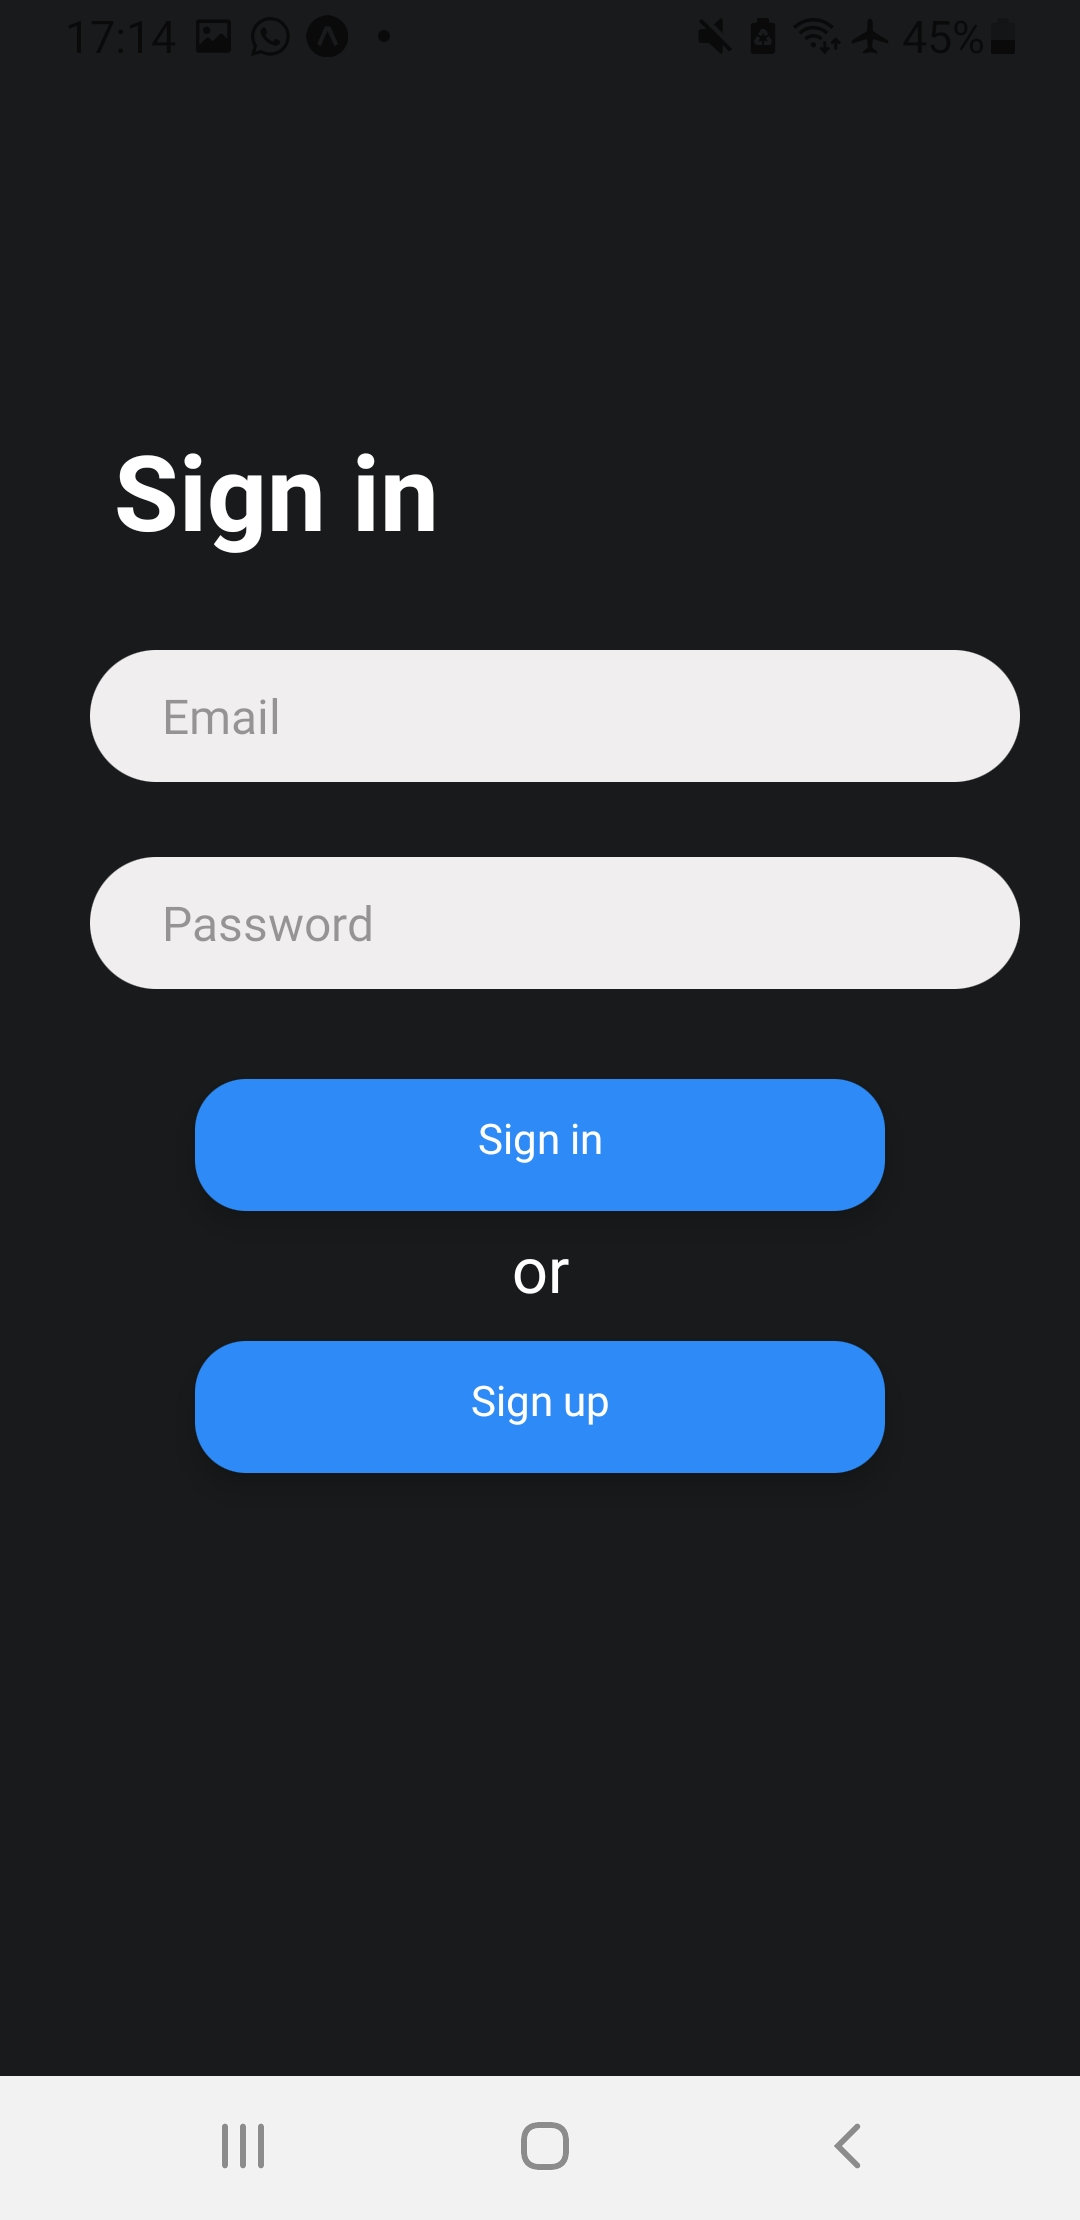
\includegraphics[width=5cm, height=10cm]{images/immaginiAndroid/signIn.jpg}
        \caption{\label{signInAndroid} Android schermo Sign In}
    \end{minipage}
    \hfill
    \begin{minipage}[h]{0.47\textwidth}
        \centering
        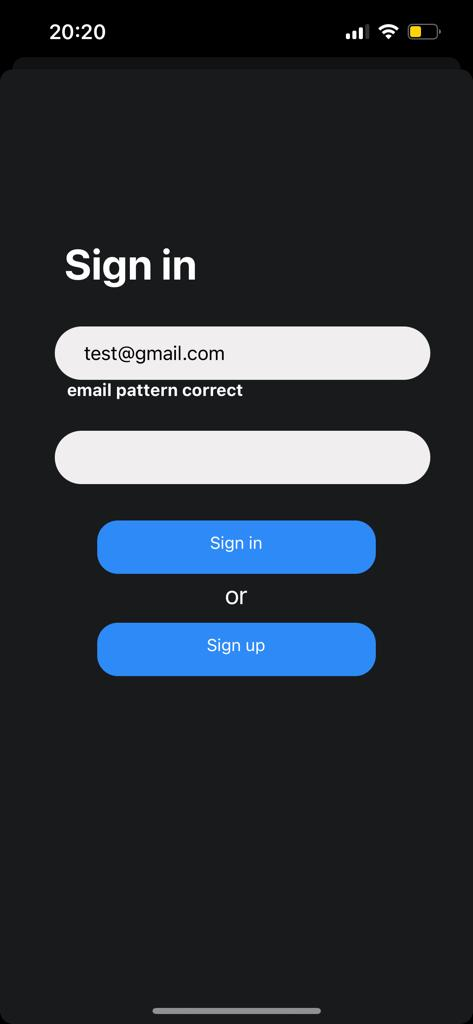
\includegraphics[width=5cm, height=10cm]{images/immaginiPhone/signIn.jpeg}
        \caption{\label{signIniPhone}iPhone schermo Sign In}
    \end{minipage}
    \begin{minipage}[h]{0.47\textwidth}
        \centering
        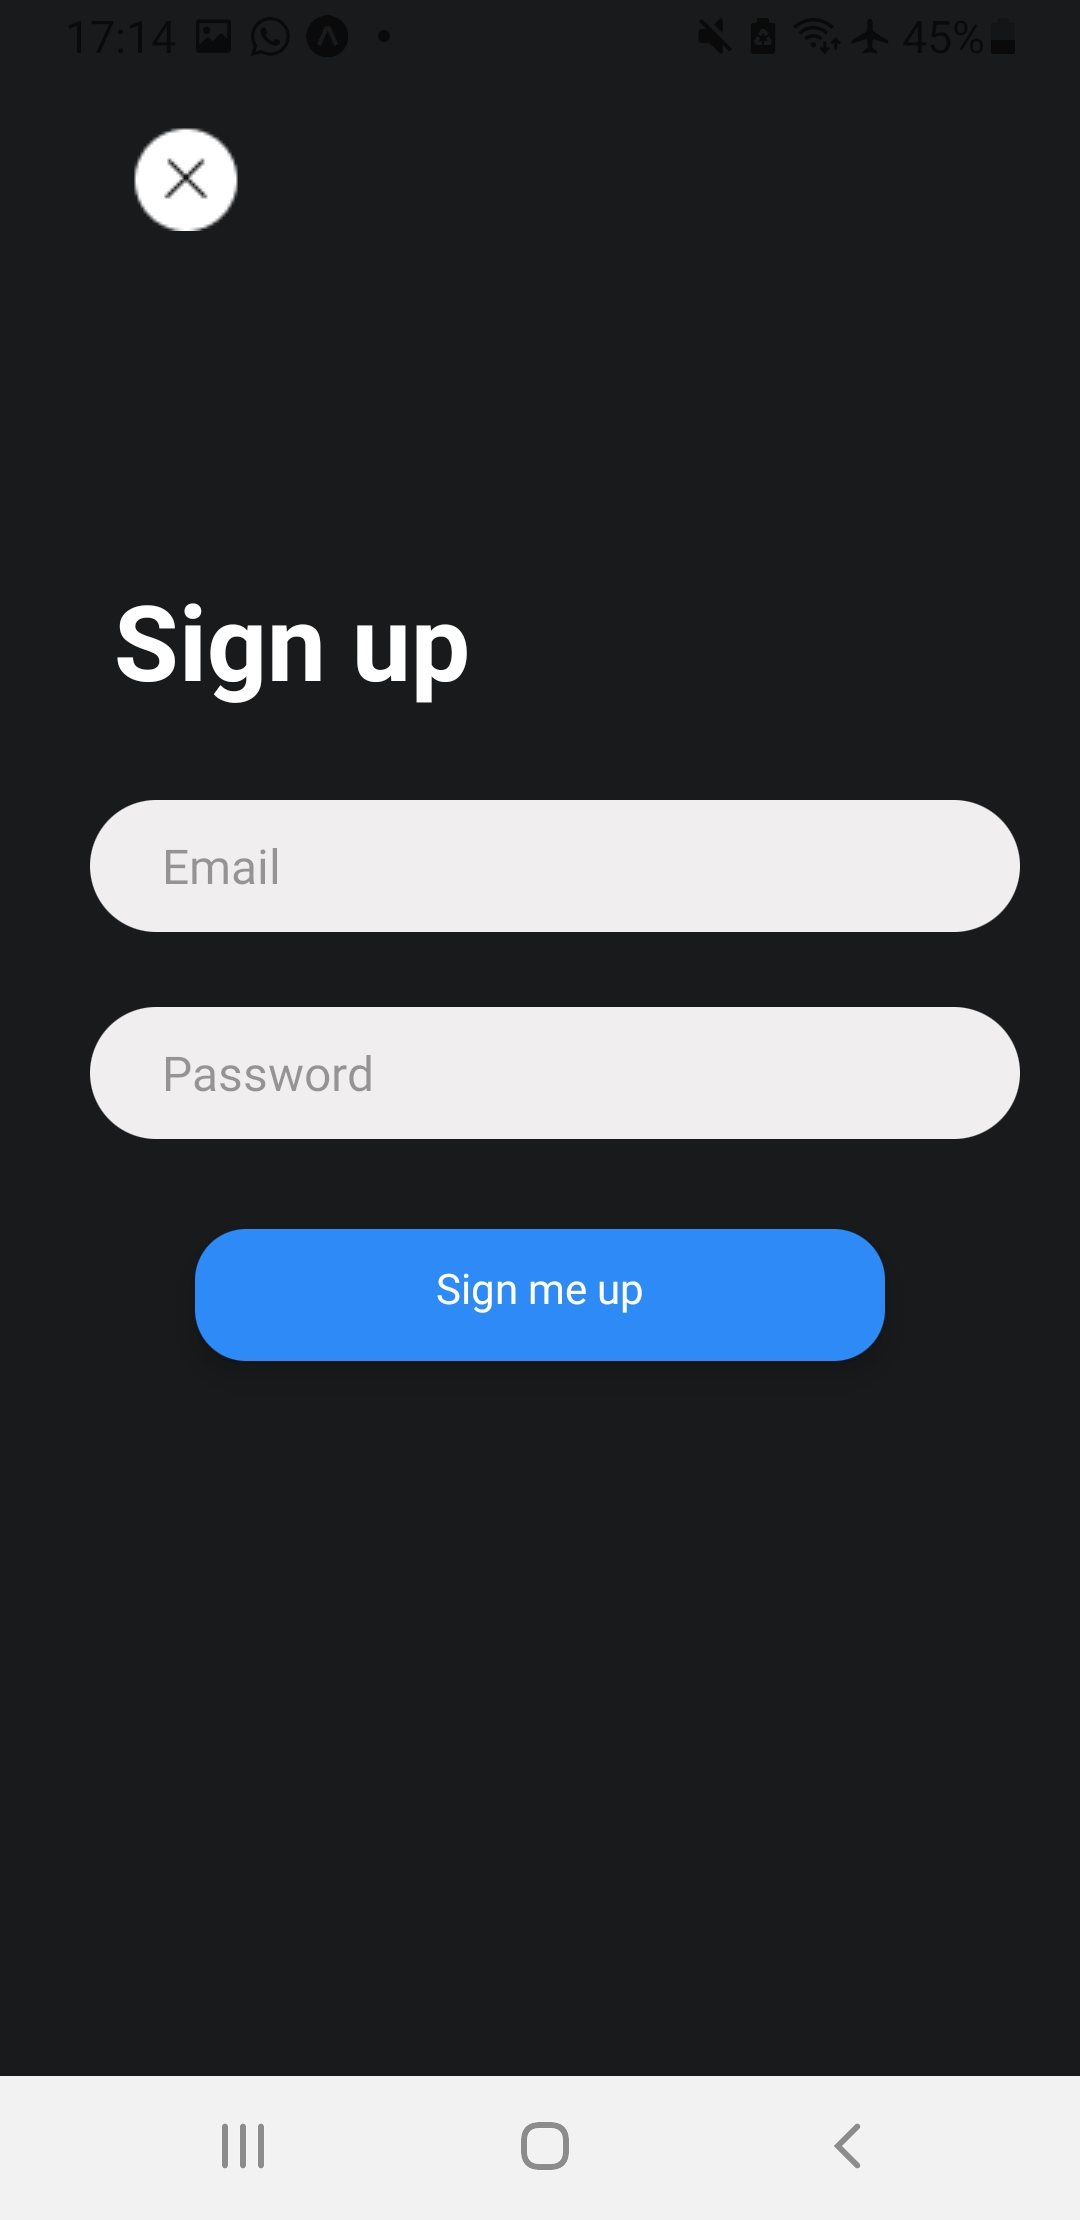
\includegraphics[width=5cm, height=10cm]{images/immaginiAndroid/signUp.jpg}
        \caption{\label{signUnAndroid} Android schermo Sign Up}
    \end{minipage}
    \hfill
    \begin{minipage}[h]{0.47\textwidth}
        \centering
        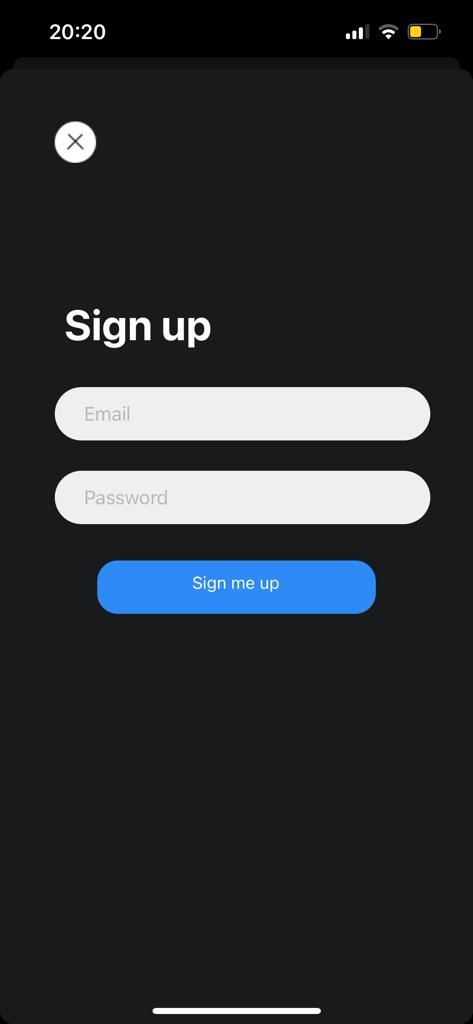
\includegraphics[width=5cm, height=10cm]{images/immaginiPhone/signUp.jpeg}
        \caption{\label{signUniPhone}iPhone schermo Sign Up}
    \end{minipage}
\end{figure}
Una volta acceduto al proprio profilo, l'utente viene reindirizzato nella schermata principale, nella quale vengono visualizzate di volta in volta le immagini ricercate.
\section{Immagini Memorizzate nella Cache}
Se l'utente ha gi\`a effettuato in precedenza l'accesso all'applicazione, nel proprio dispotivo \`e gi\`a stato memorizzato un JWT;
essendo gi\`a in possesso di questo oggetto l'utente viene reindirizzato dallo Splash Screen allo screen destinato alle immagini memorizzate nella Cache. Tale schermo \`e mostrato
nella Fig 4.7 (4.8 per iPhone) e mostra le ultime immagini che l'utente ha visualizzato prima di chiudere l'applicazione.
\begin{figure}[h]
    \begin{minipage}[h]{0.47\textwidth}
        \centering
        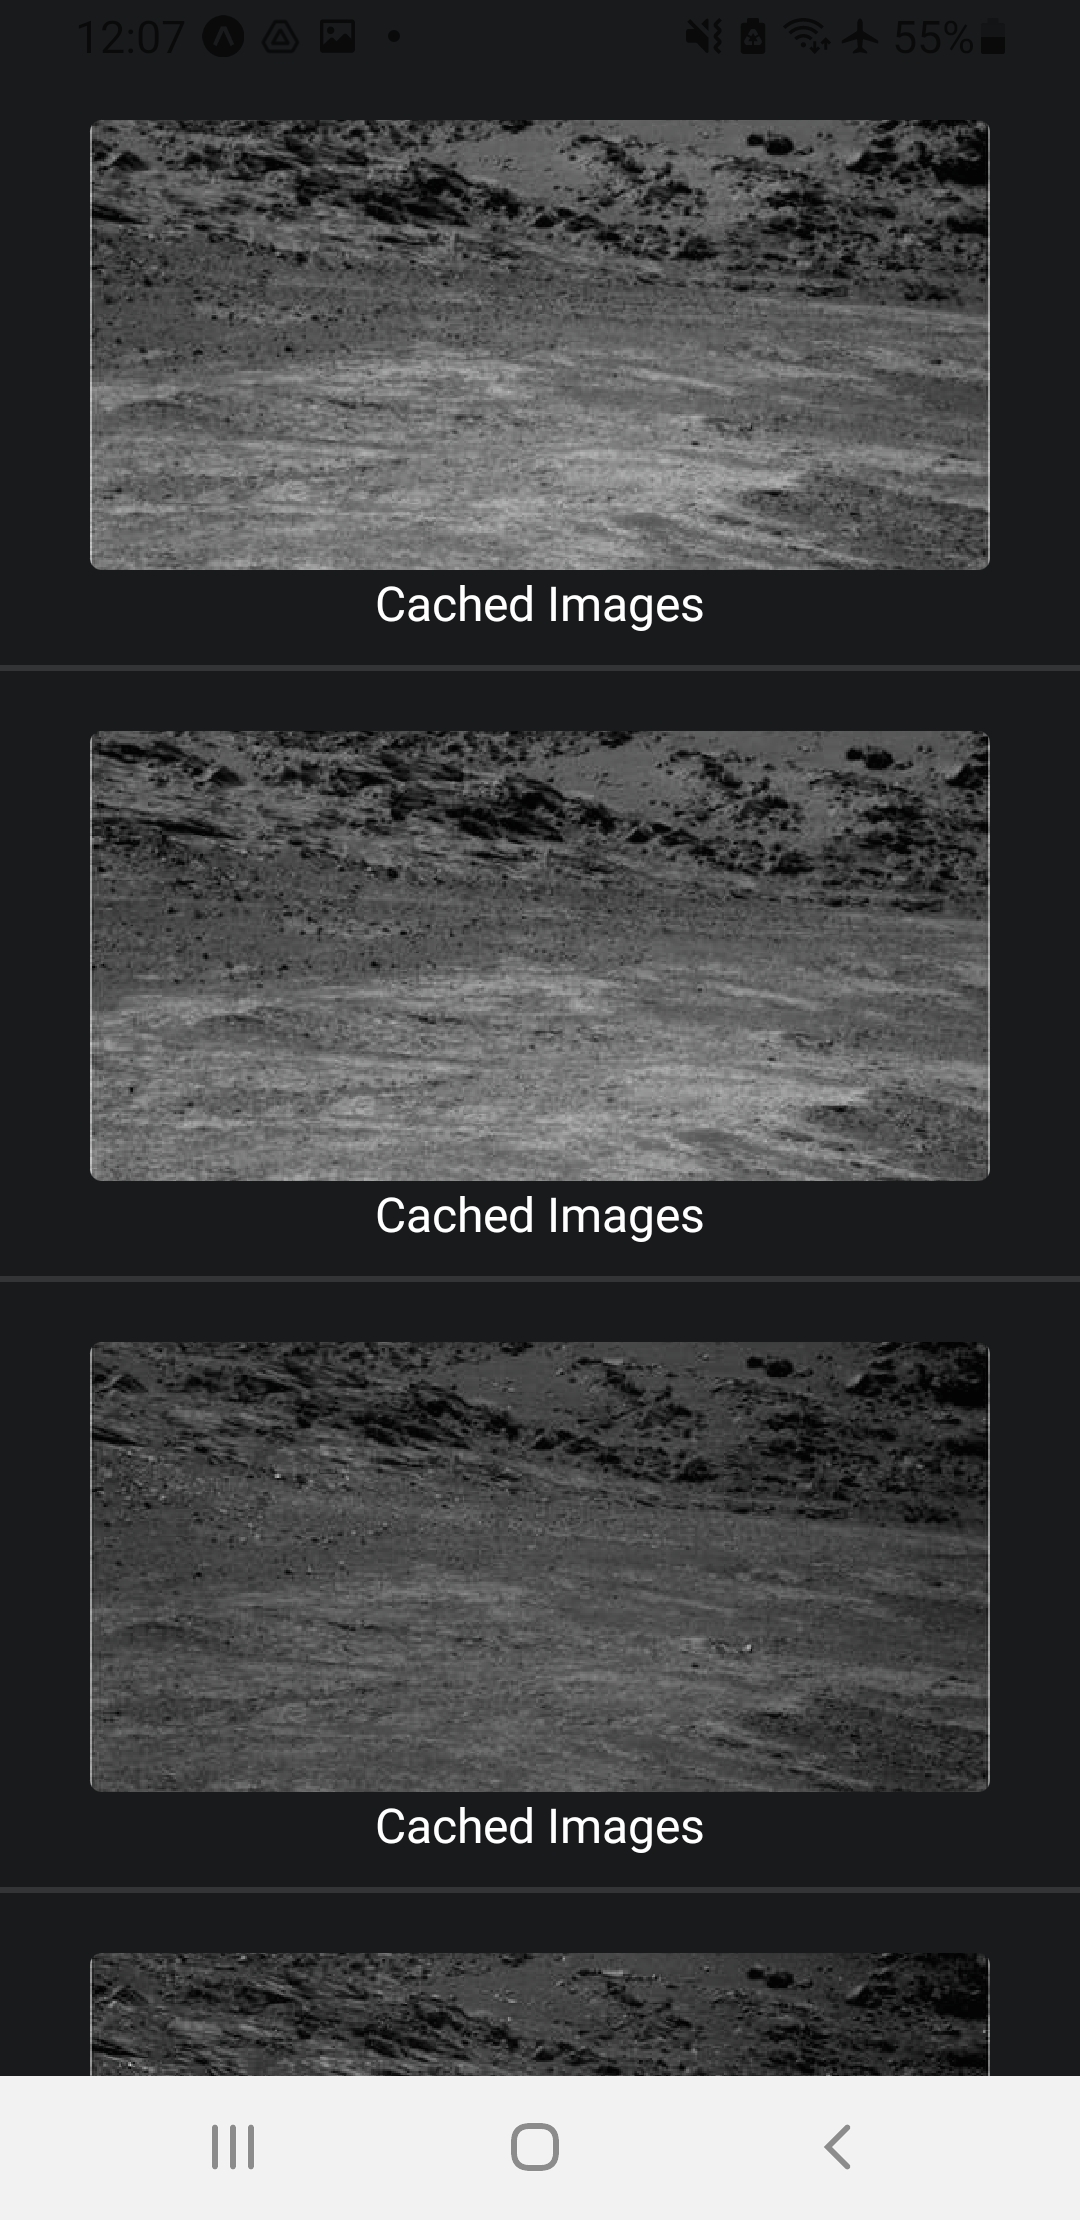
\includegraphics[width=5cm, height=10cm]{images/immaginiAndroid/imagesLoadin.jpg}
        \caption{\label{imagesLoadinAndroid} Android schermo per immagini memorizzate in cache}
    \end{minipage}
    \hfill
    \begin{minipage}[h]{0.47\textwidth}
        \centering
        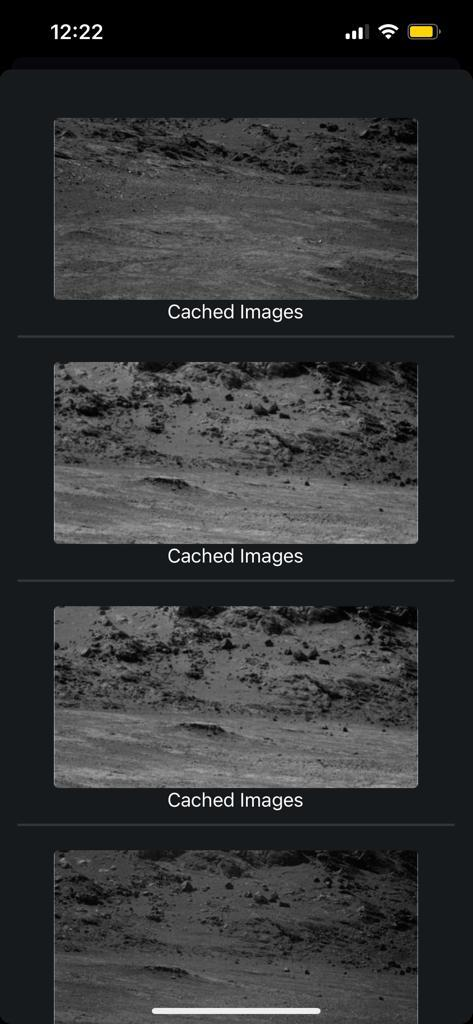
\includegraphics[width=5cm, height=10cm]{images/immaginiPhone/imagesLoading.jpeg}
        \caption{\label{imagesLoadinIphone}iPhone schermo per immagini memorizzate in cache}
    \end{minipage}
\end{figure}

Dalle Fig 4.7 e 4.8 si pu\`o evincere che l'unica differenza tra Android e iPhone \`e una maggiore distanza dall'header dello schermo.
\section{Ricerca Immagini per Nome Rover}
Per poter ricercare le immagini tramite il nome del Rover, l'utente deve:

\begin{enumerate}
    \item Assicurarsi che il pulsante ``All" non sia stato premuto, quindi sia di colore grigio.
    \item Digitare uno dei tre nomi possibili nella Search-Bar: Curiosity, Opportunity e Spirit.
    \item Cliccare sul pulsante ``All" avviando la ricerca.
\end{enumerate}

\begin{figure}[h]
    \begin{minipage}[h]{0.47\textwidth}
        \centering
        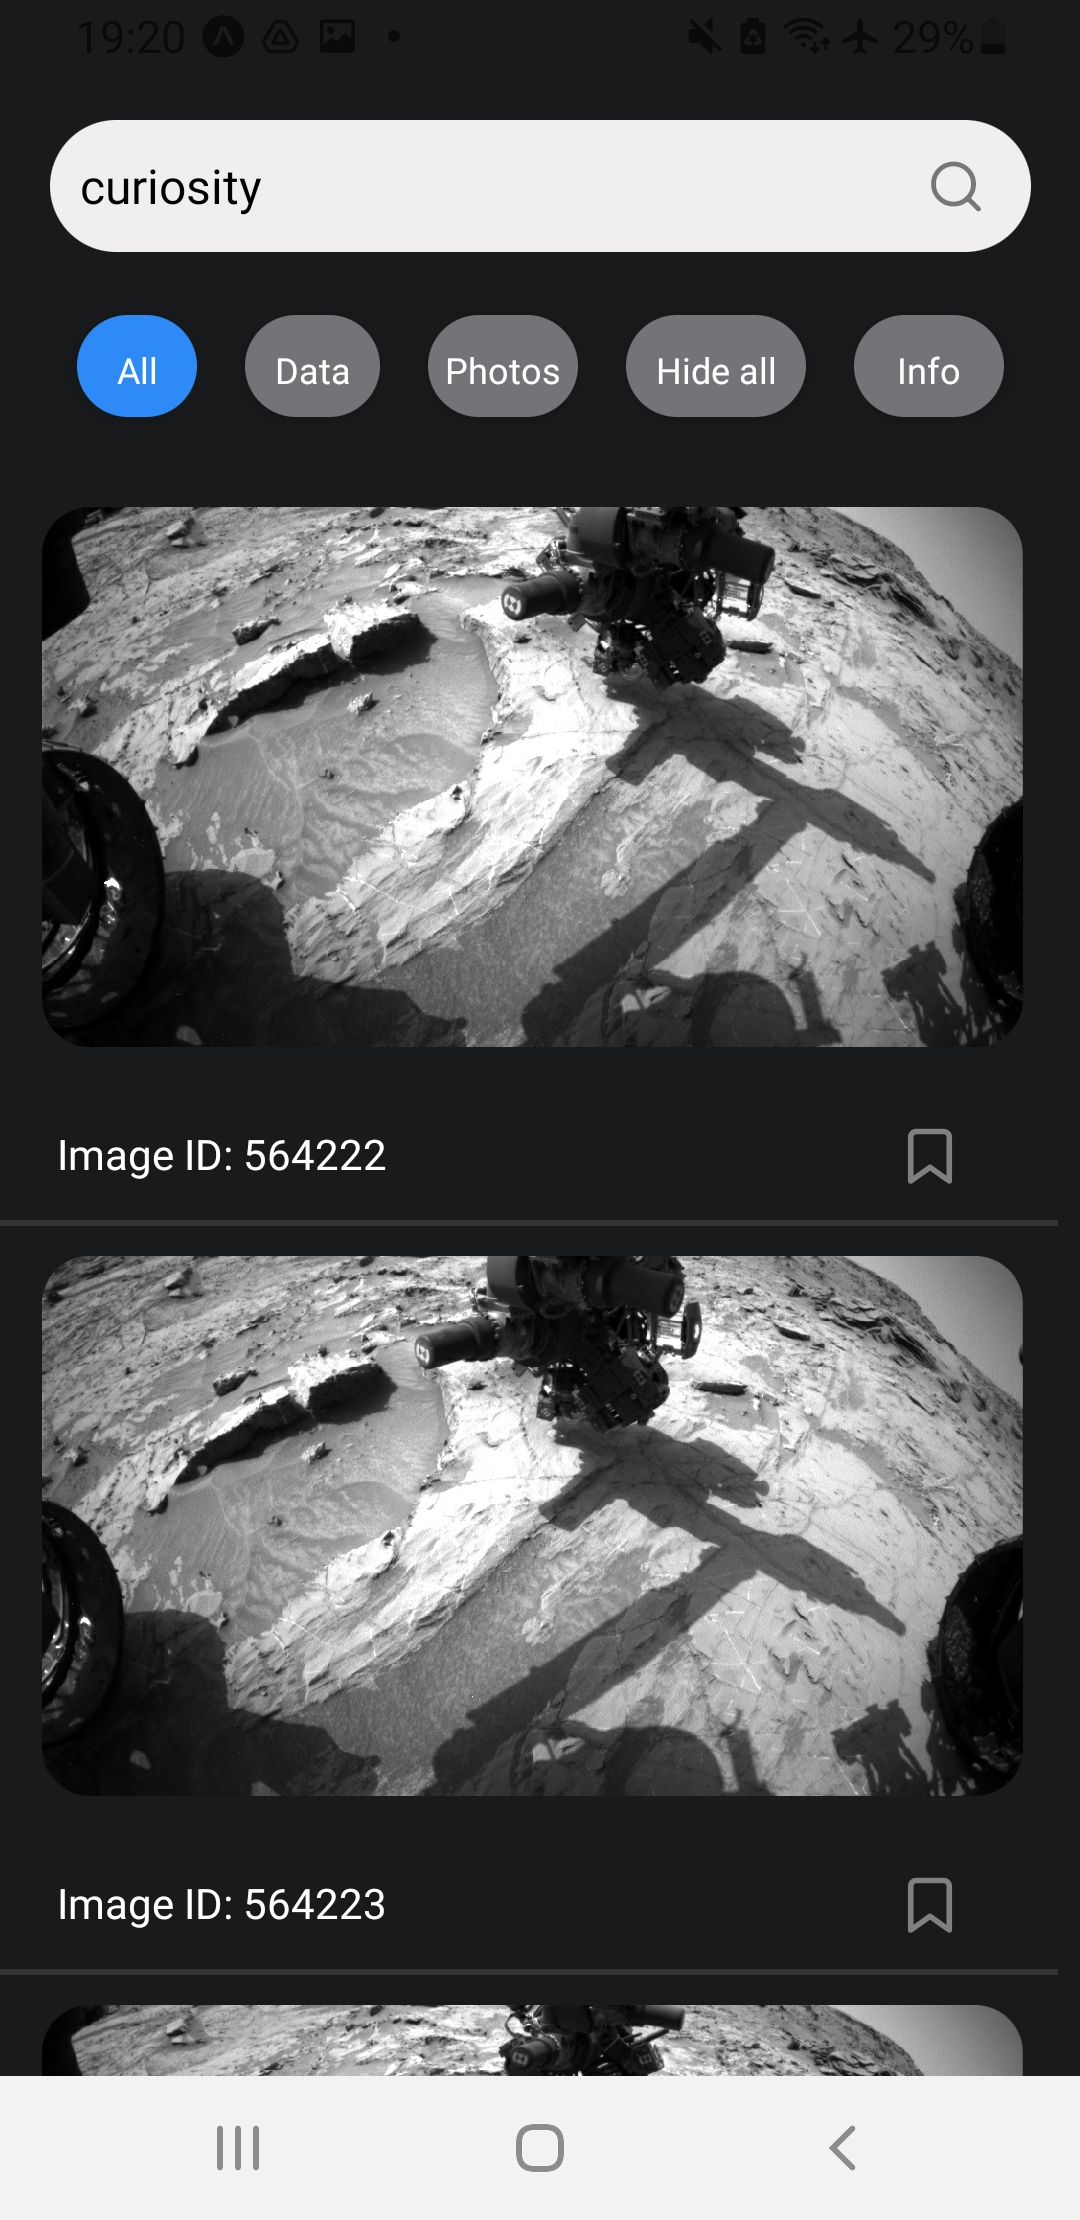
\includegraphics[width=5cm, height=10cm]{images/immaginiAndroid/ricercaNomeRover.jpg}
        \caption{\label{ricercaNomeRoverAndroid} Android ricerca per nome}
    \end{minipage}
    \hfill
    \begin{minipage}[h]{0.47\textwidth}
        \centering
        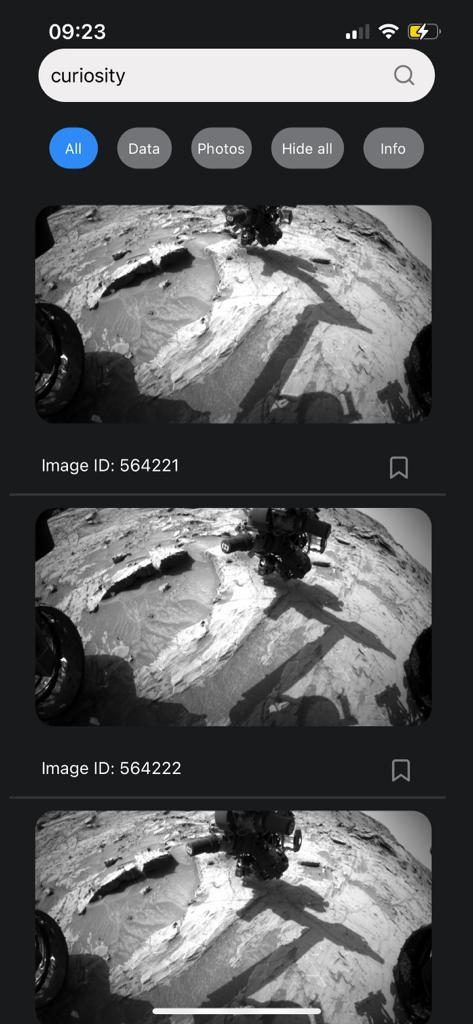
\includegraphics[width=5cm, height=10cm]{images/immaginiPhone/ricercaNomeRover.jpeg}
        \caption{\label{ricercaNomeRoverIphone}iPhone ricerca per nome}
    \end{minipage}
\end{figure}

Dalla Fig 4.9 e 4.10 non si nota nessuna differenza tra i due dispositivi: per la realizzazione di questi screen \`e stato infatti utilizzato uno stile di
presentazione chiamato ``FlexBox", il quale si adatta ai vari dispositivi su cui \`e utilizzato.

\section{Ricercare Immagini per Data Solare}
Per ricercare immagini per data solare l'utente deve premere il pulsante ``data" in modo da essere reindirizzato nello screen mostrato nella Fig 4.11 (4.12 per iPhone).
In questa schermata si possono inserire giorno, mese e anno in cui sono state scattate le immagini e premere su ``Search by date" per iniziare la ricerca.
\begin{figure}[h]
    \begin{minipage}[h]{0.47\textwidth}
        \centering
        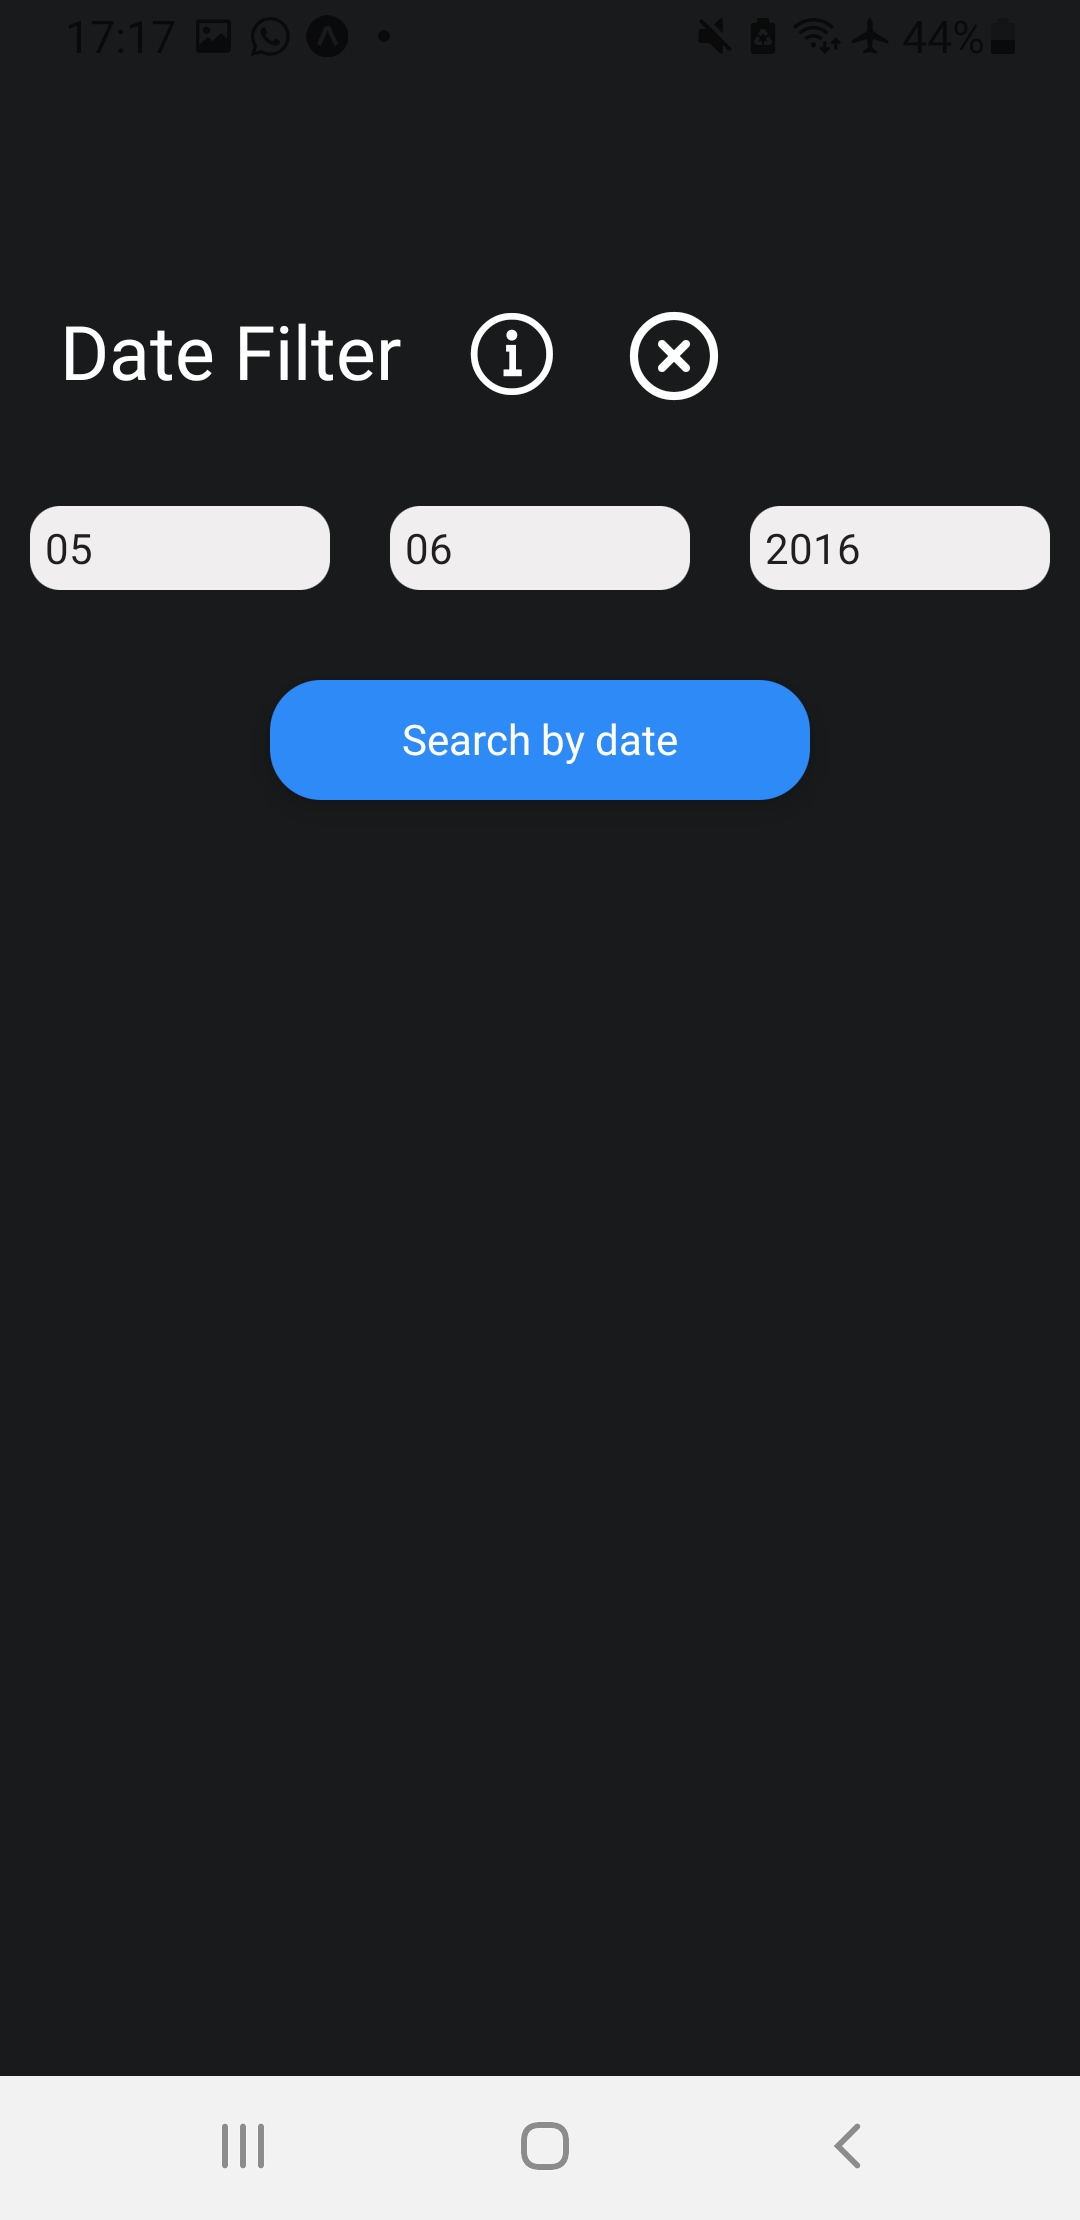
\includegraphics[width=5cm, height=10cm]{images/immaginiAndroid/SearchbyDate.jpg}
        \caption{\label{SearchbyDateAndroid} Android ricerca per data solare}
    \end{minipage}
    \hfill
    \begin{minipage}[h]{0.47\textwidth}
        \centering
        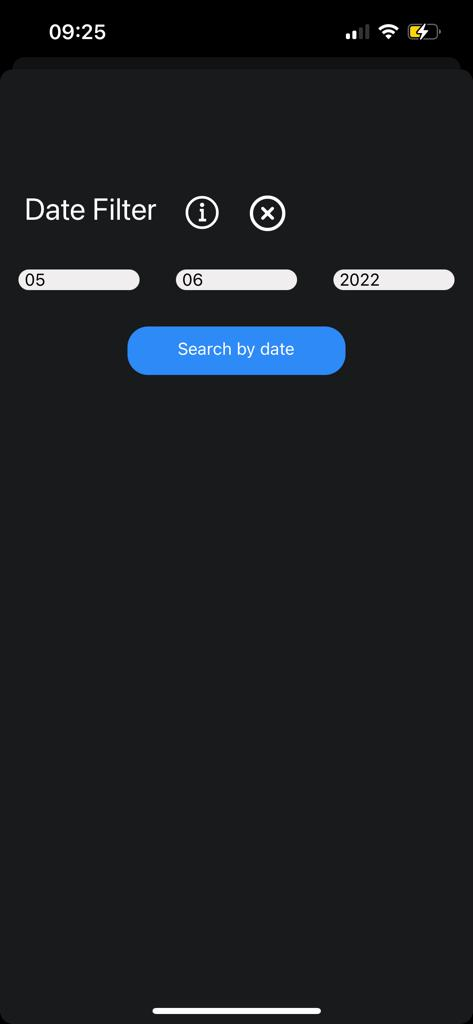
\includegraphics[width=5cm, height=10cm]{images/immaginiPhone/SearchbyDate.jpeg}
        \caption{\label{SearchbyDateIphone}iPhone ricerca per data solare}
    \end{minipage}
\end{figure}

Osservando attentamente le Fig 4.11 e 4.12 si possono notare due principali differenze tra i due dispositivi:
\begin{itemize}
    \item I campi dove l'utente pu\`o digitare il testo sono diversi, in quanto il componente TextInput di React Native viene reindirizzato in un componente nativo diverso a seconda della piattaforma di destinazione \cite{ReactNativeComponent}.
    \item Il pulsante ``Search by date" \`e diverso per lo stesso motivo descritto sopra.
\end{itemize}

\section{Dettagli delle Immagini}
Oltre a poter ricercare delle immagini \`e possibile visualizzare i dettagli di esse, come: l'ID del Rover, il nome del Rover e la camera che ha scattato la foto.
Per poter accedere ai dettagli di ogni immagine \`e necessario premere su una di esse, in modo da essere reindirizzati nello screen mostrato nella Fig 4.13 (4.14 per iOS).
In questo screen oltre a poter vedere i dettagli di una immagine \`e anche possibile nascondere la stessa premendo sul pulsante ``Hide this image".
Una volta occultata, l'immagine non viene pi\`u mostrata nella schermata principale a meno che l'utente non prema il pulsante ``Photos".

Osservando le Fig 4.13 e 4.14 possiamo notare alcune differenze tra i due dispositivi:
\begin{enumerate}
    \item Il pulsante ``Hide this image" viene presentato in modo diverso poich\`e il componente Button di React Native viene reindirizzato differentemente a seconda della piattaforma di destinazione \cite{ReactNativeComponent}.
    \item L'icona rappresentata con una ``X" si trova in due posizioni diverse sui dispositivi; in iOS \`e molto vicino all'Header dello schermo, mentre in Android si trova pi\`u in basso. Questa differenza di locazione
          \`e dovuta al fatto che l'icona \`e stata posizionata utilizzando come dimensione i pixel dello schermo e quindi non \`e responsive rispetto alle dimensioni di ogni dispotivo.
\end{enumerate}

\begin{figure}[h]
    \begin{minipage}[h]{0.47\textwidth}
        \centering
        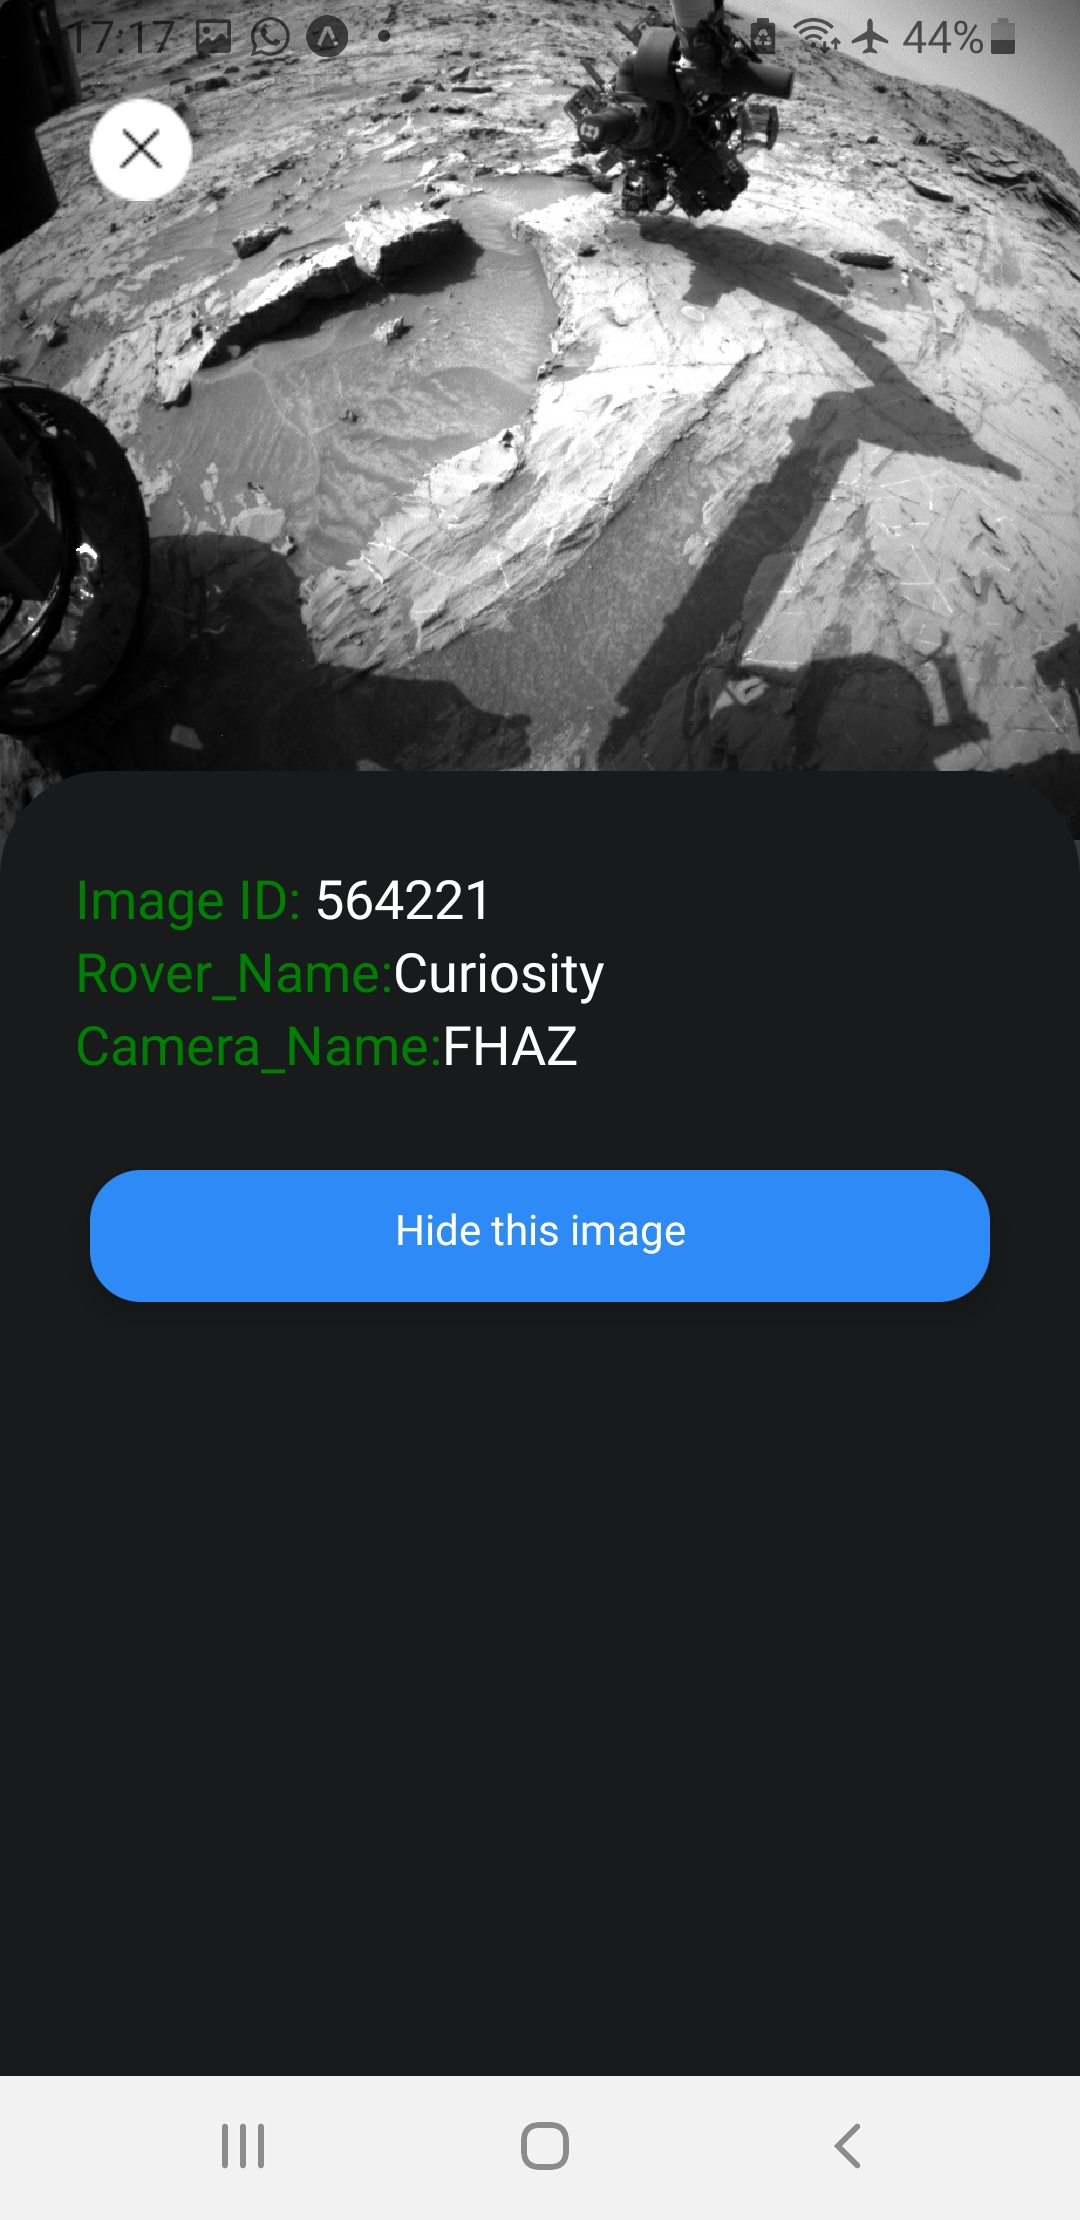
\includegraphics[width=5cm, height=10cm]{images/immaginiAndroid/imageDetail.jpg}
        \caption{\label{imageDetailAndroid} Android dettagli immagine}
    \end{minipage}
    \hfill
    \begin{minipage}[h]{0.47\textwidth}
        \centering
        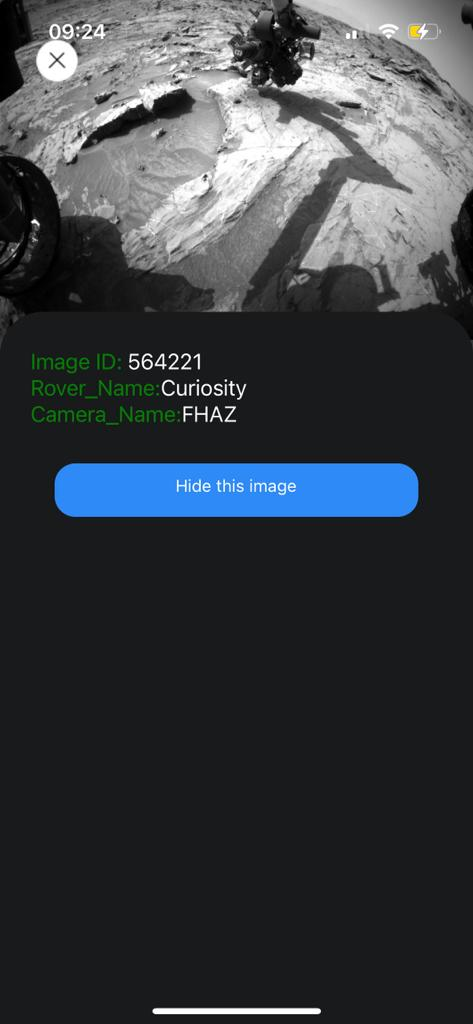
\includegraphics[width=5cm, height=10cm]{images/immaginiPhone/imageDetail.jpeg}
        \caption{\label{imageDetailIphone}iPhone dettagli immagine}
    \end{minipage}
\end{figure}

\section{Filtri Photos e Hide All}
Una volta nascoste le immagini, queste non vengono mostrate all'utente quando effettua una ricerca: possono per\`o essere ripristinate tramite l'utilizzo del filtro ``Photos".
Nella Fig 4.15 si pu\`o notare che l'immagine con ID=564234 non \`e visibile prima di premere il pulsante ``Photos"; questa viene visualizzata dopo averlo premuto.

All'utente viene fornita la possibilit\`a di nascondere tutti gli elementi di una ricerca premendo il pulsante ``Hide All".
\begin{figure}[h]
    \begin{minipage}[h]{0.47\textwidth}
        \centering
        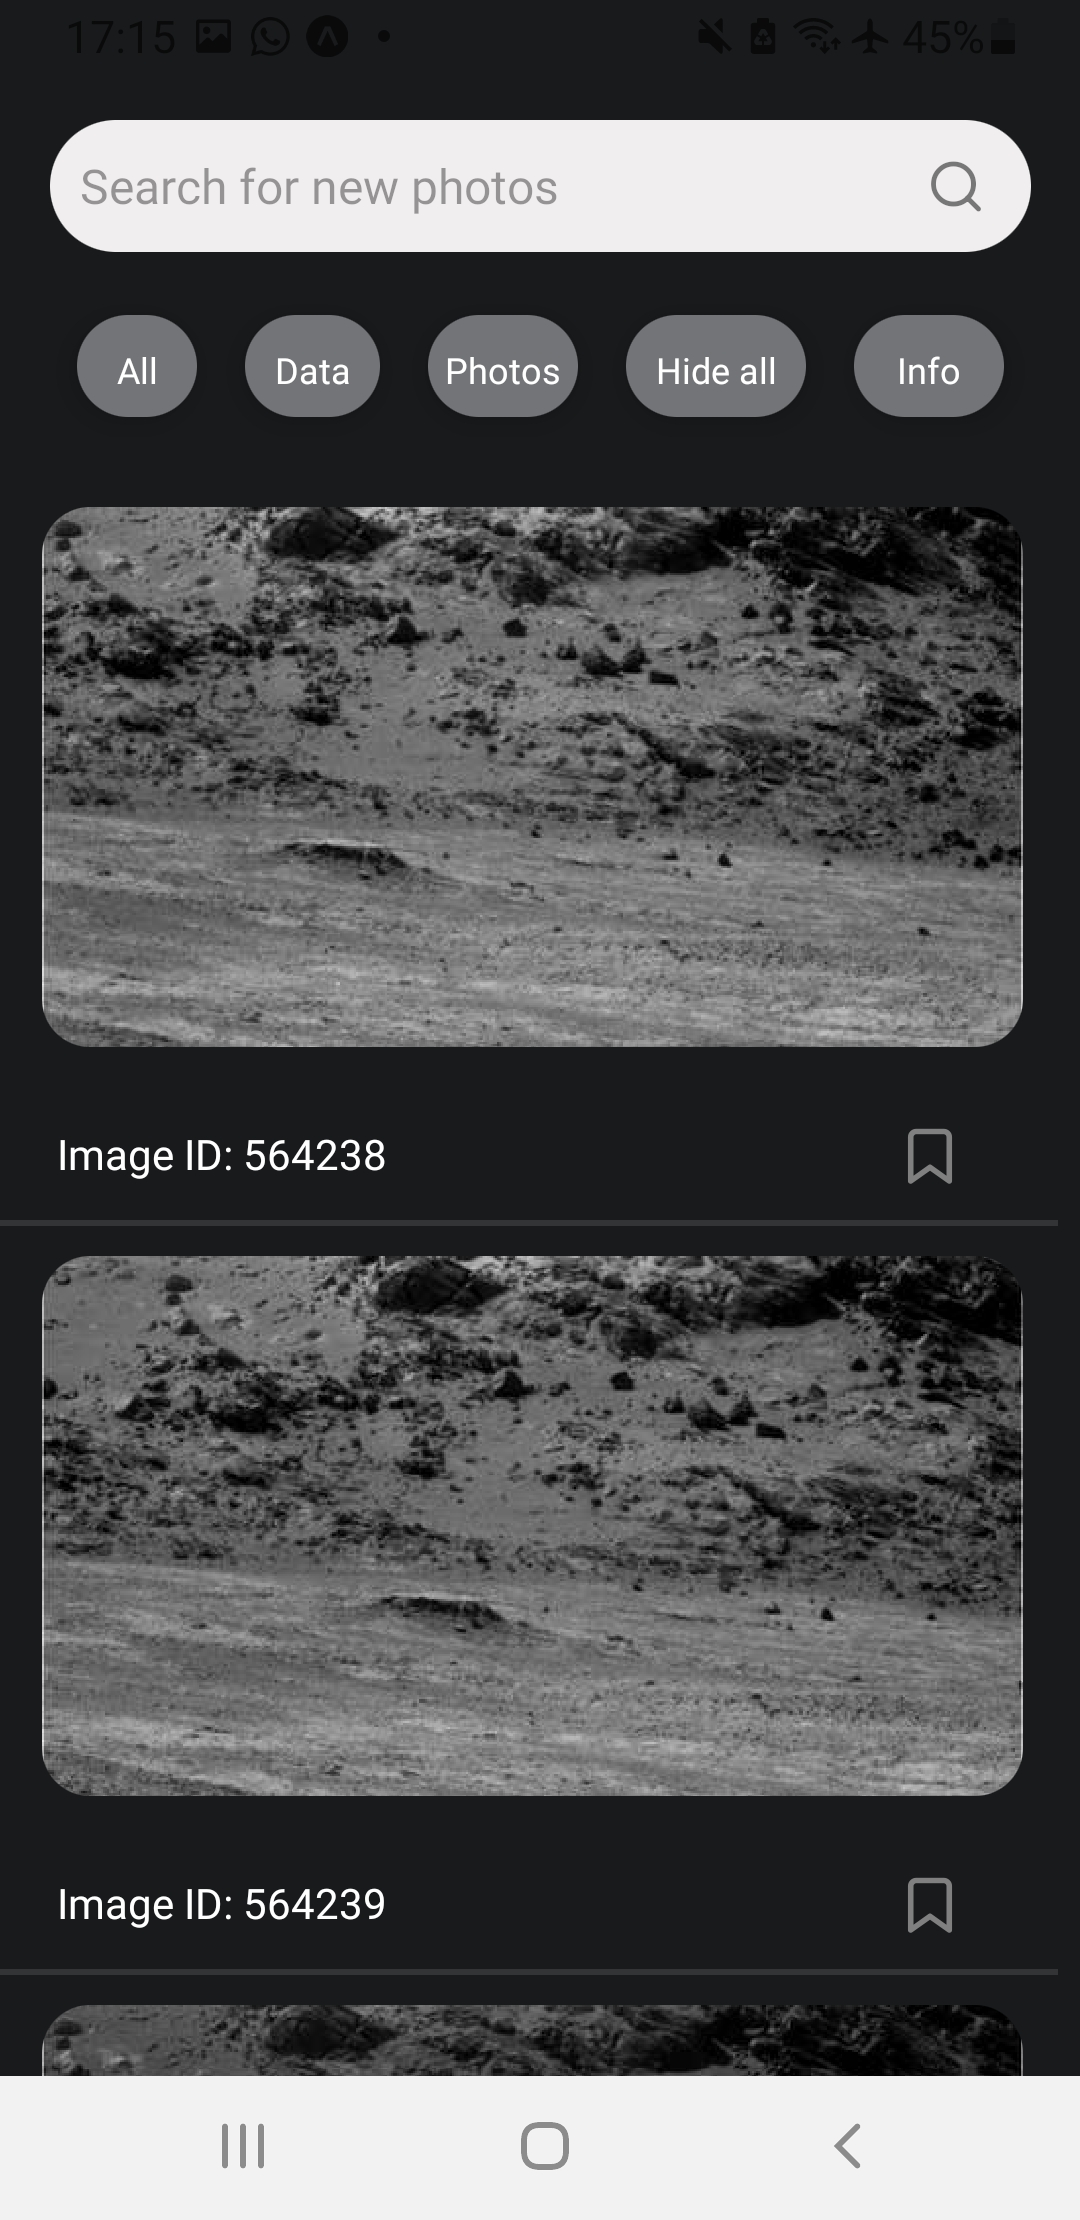
\includegraphics[width=5cm, height=10cm]{images/immaginiAndroid/prePhotos.jpg}
        \caption{\label{prePhotosAndroid} Lista delle immagini prima di usare il filtro Photos}
    \end{minipage}
    \hfill
    \begin{minipage}[h]{0.47\textwidth}
        \centering
        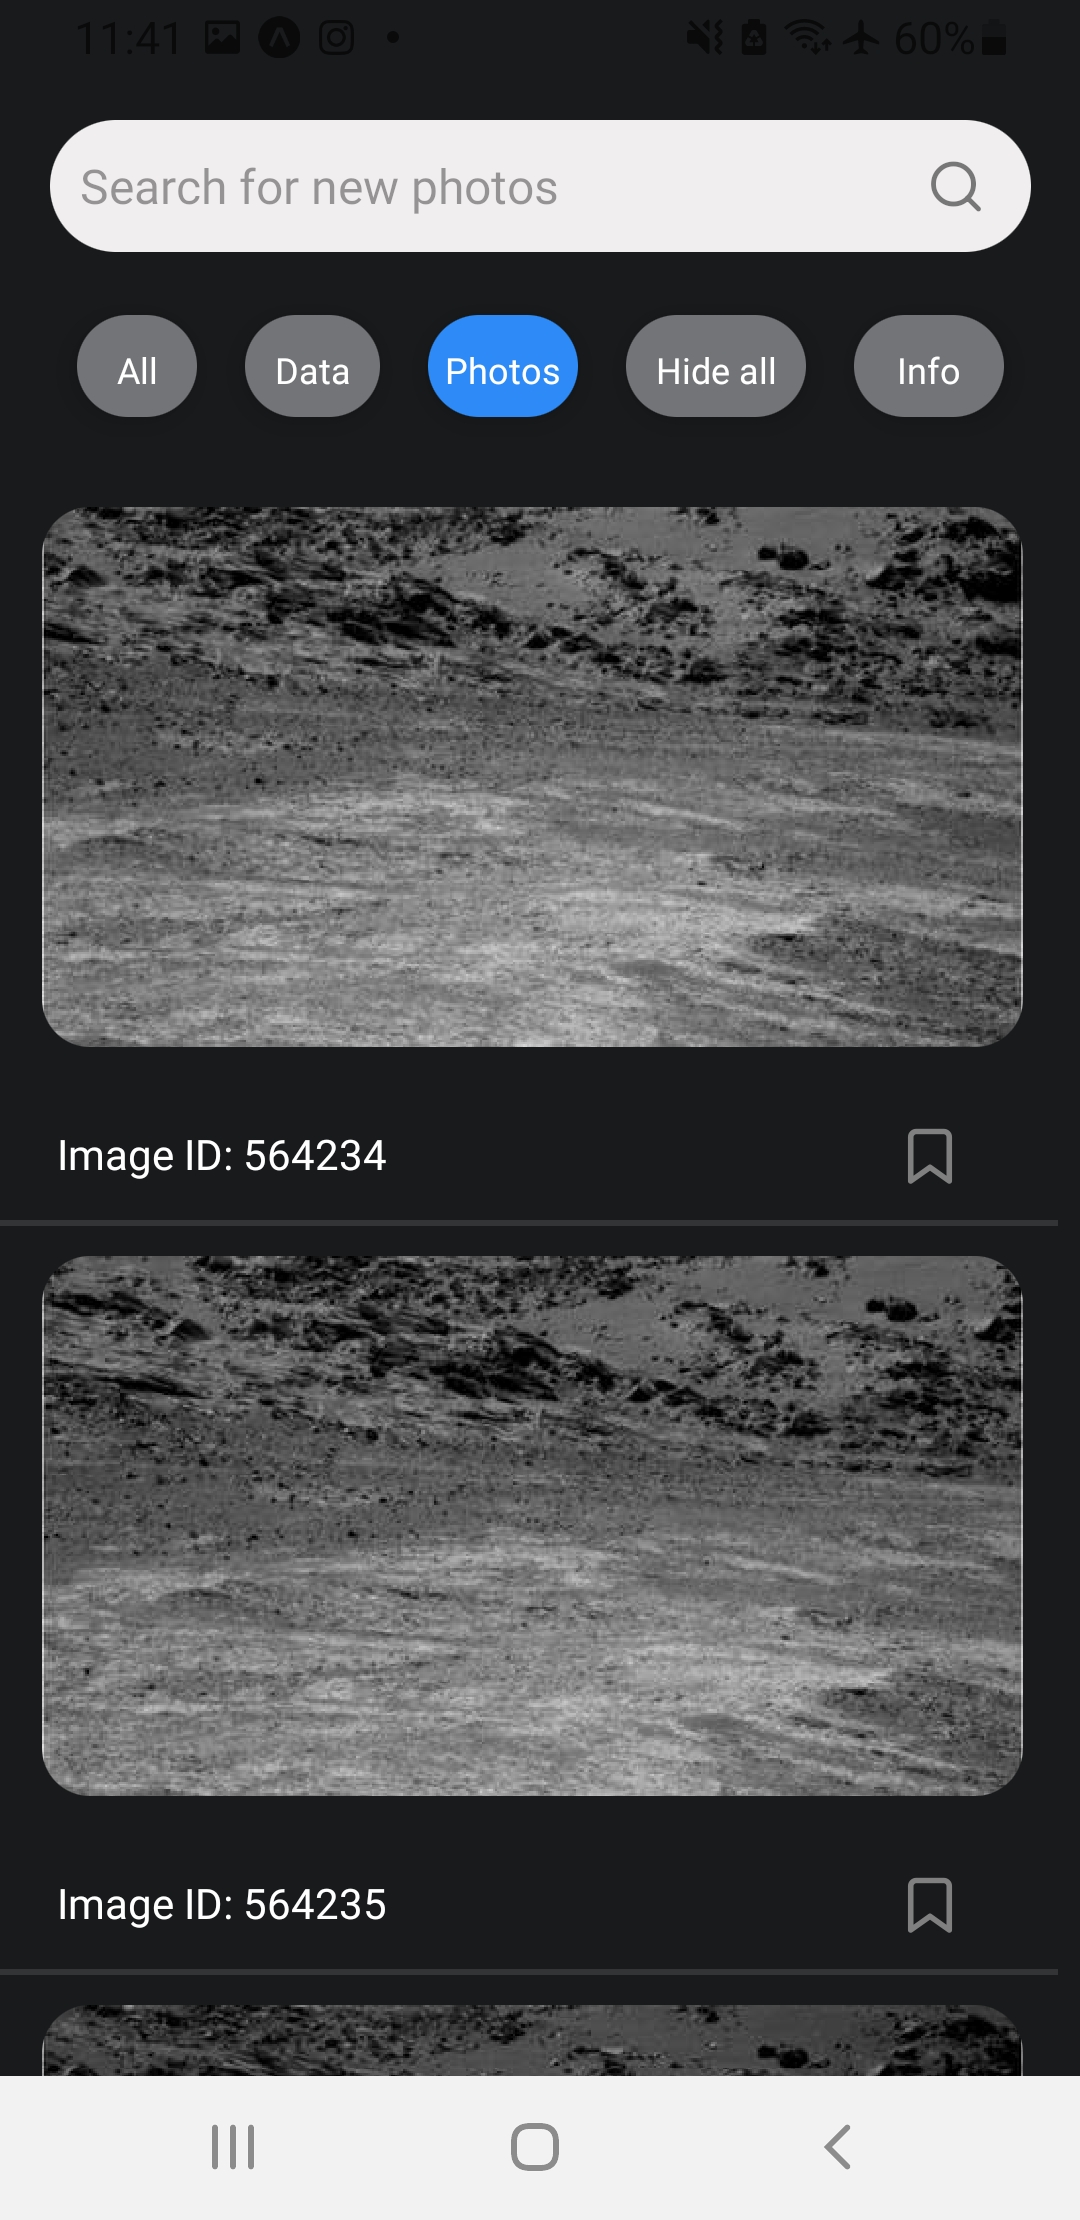
\includegraphics[width=5cm, height=10cm]{images/immaginiAndroid/postPhotos.jpg}
        \caption{\label{postPhotosAndroid} Lista delle immagini dopo l'uso del filtro Photos}
    \end{minipage}
\end{figure}
\section{Parametri di Ricerca Errati}
Quando l'utente effettua una nuova ricerca di immagini, potrebbe inserire dei parametri di ricerca errati come ad esempio il nome del Rover errato e la data solare in formato errato;
in tal caso nessuna immagine viene recuperata. In queste situazioni l'applicativo si occupa di informare l'utente del fatto che nessuna immagine \`e
stata trovata e viene visualizzata a schermo una lista vuota.

Osservando le Fig 4.17 e 4.18 possiamo notare che le visualizzazione delle modali non cambia tra Android e iOS; l'unica differenza percepibile nei due dispositivi consiste in un testo pi\`u marcato in Android.
\begin{figure}[h]
    \begin{minipage}[h]{0.47\textwidth}
        \centering
        \includegraphics[width=5cm, height=10cm]{images/immaginiAndroid/ricercaErrata.jpg}
        \caption{\label{ricercaErrataAndroid} Android ricerca errata}
    \end{minipage}
    \hfill
    \begin{minipage}[h]{0.47\textwidth}
        \centering
        \includegraphics[width=5cm, height=10cm]{images/immaginiPhone/ricercaErrata.jpeg}
        \caption{\label{ricercaErrataIphone} iPhone ricerca errata}
    \end{minipage}
\end{figure}

\section{Animazione Onde Gravitazionali}
Ogni volta che viene eseguita una nuova ricerca, dopo aver premuto il pulsante ``All", viene avviata una animazione. In questo modo l'utente ha una migliore UX (User Experience) in quanto viene informato che la ricerca \`e inziziata e l'animazione ricorda le onde gravitazionali, quindi lo spazio.
\begin{figure}[H]
    \begin{minipage}[h]{0.47\textwidth}
        \centering
        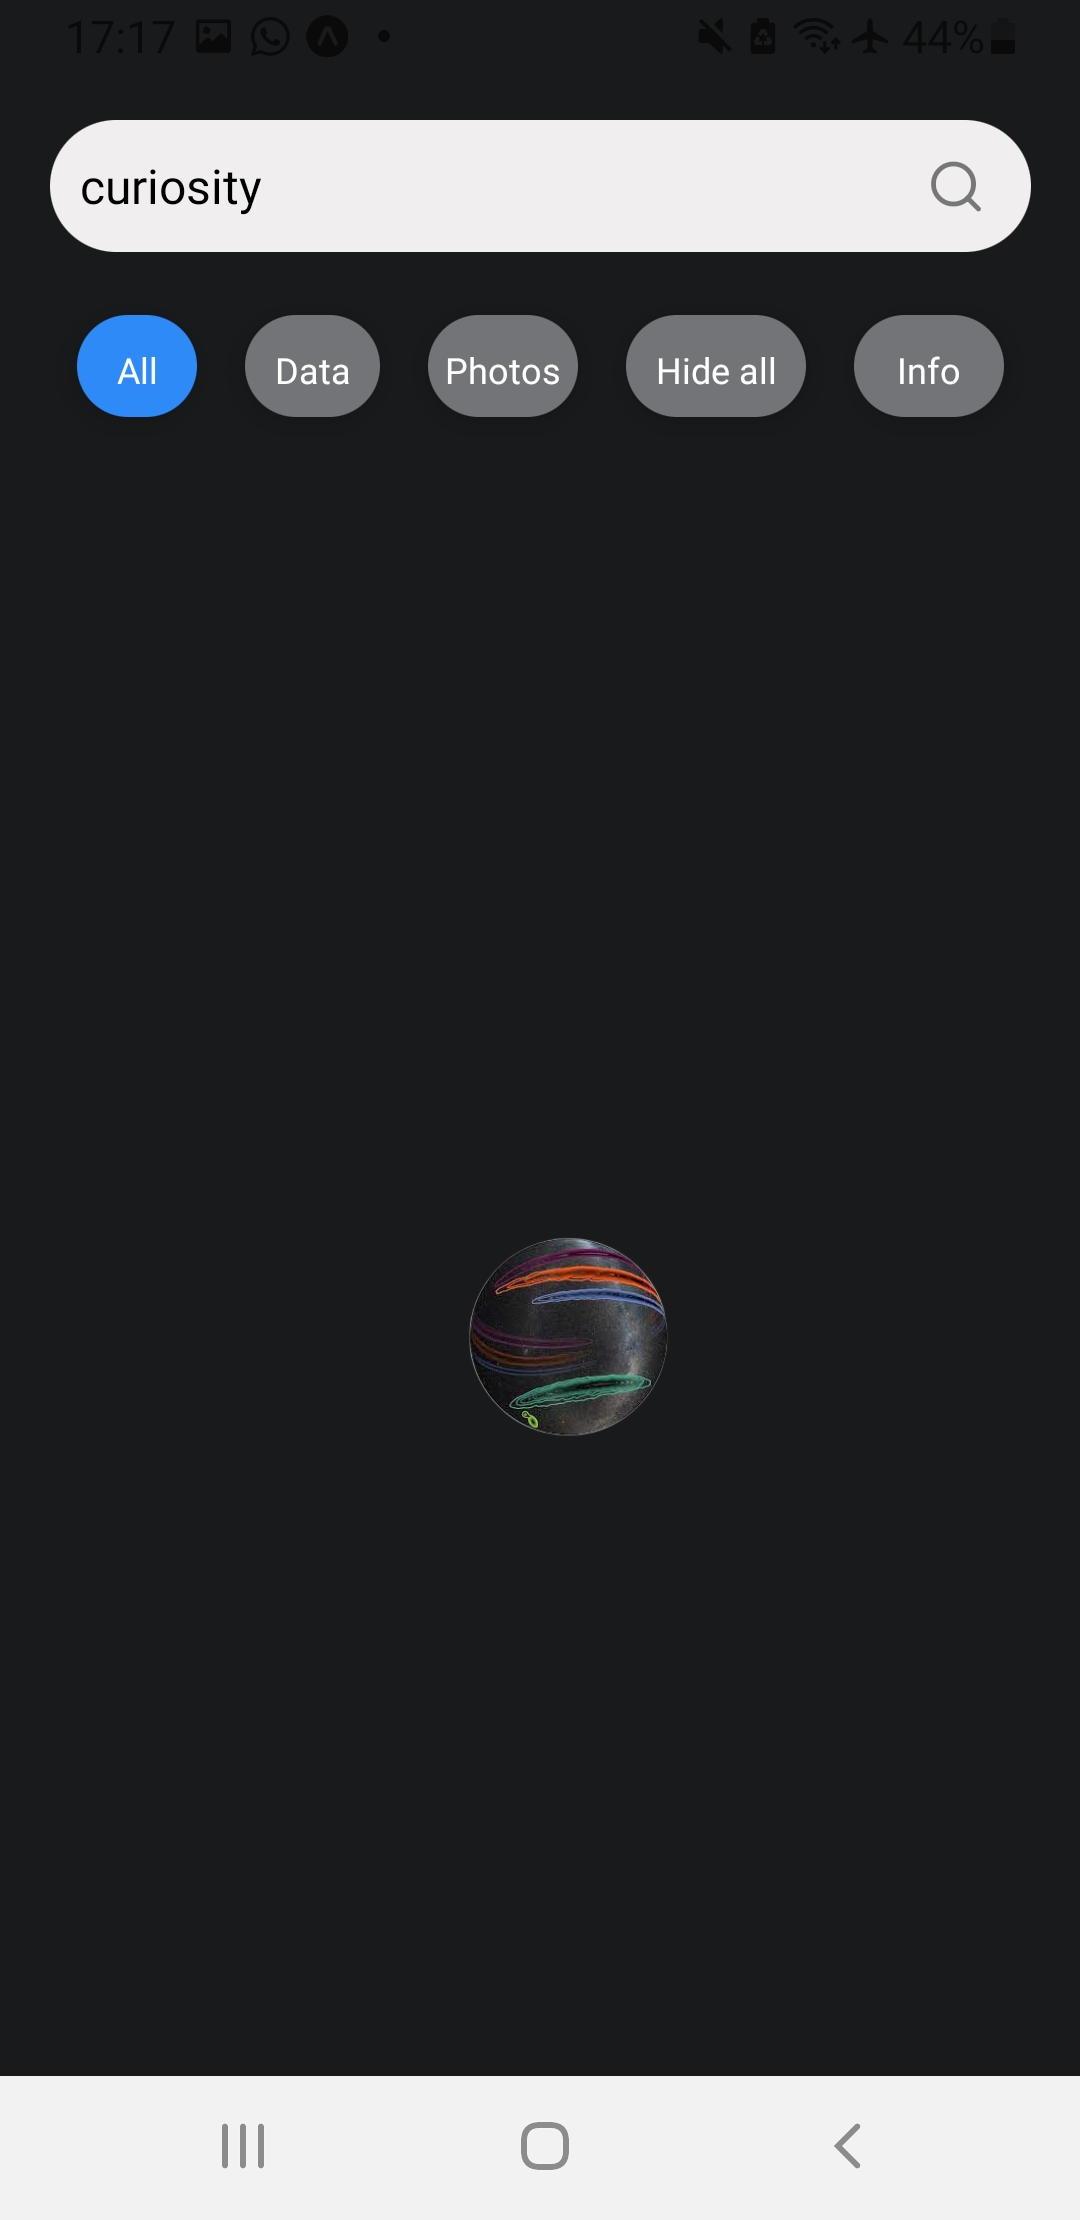
\includegraphics[width=5cm, height=10cm]{images/immaginiAndroid/animazione.jpg}
        \caption{\label{animazioneAndroid} Android animazione onde gravitazionali}
    \end{minipage}
    \hfill
    \begin{minipage}[h]{0.47\textwidth}
        \centering
        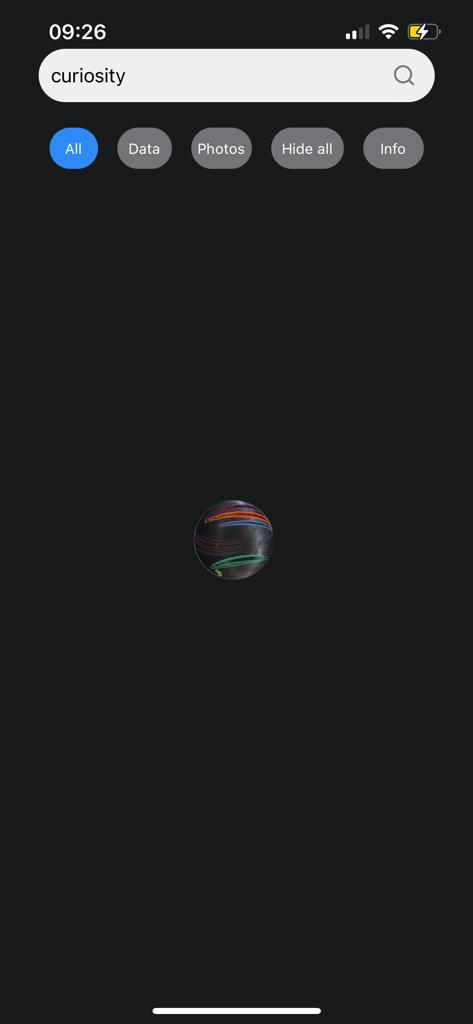
\includegraphics[width=5cm, height=10cm]{images/immaginiPhone/animazione.jpeg}
        \caption{\label{animazioneIphone} iPhone animazione onde gravitazionali}
    \end{minipage}
\end{figure}

\section{Istruzioni sui Metodi di Ricerca}
Affinch\`e l'utente possa utilizzare correttamente l'applicazione, nello screen principale e in quello dedicato alla ricerca per data solare, sono state inserite dello icone ``info-point".
Queste ultime se premute mostrano delle modali che istruiscono l'utente sul corretto uso dell'applicativo. Come gi\`a detto in precendenza la presentazione visiva delle modali non cambia tra iOS e Android.
\begin{figure}[H]
    \begin{minipage}[h]{0.47\textwidth}
        \centering
        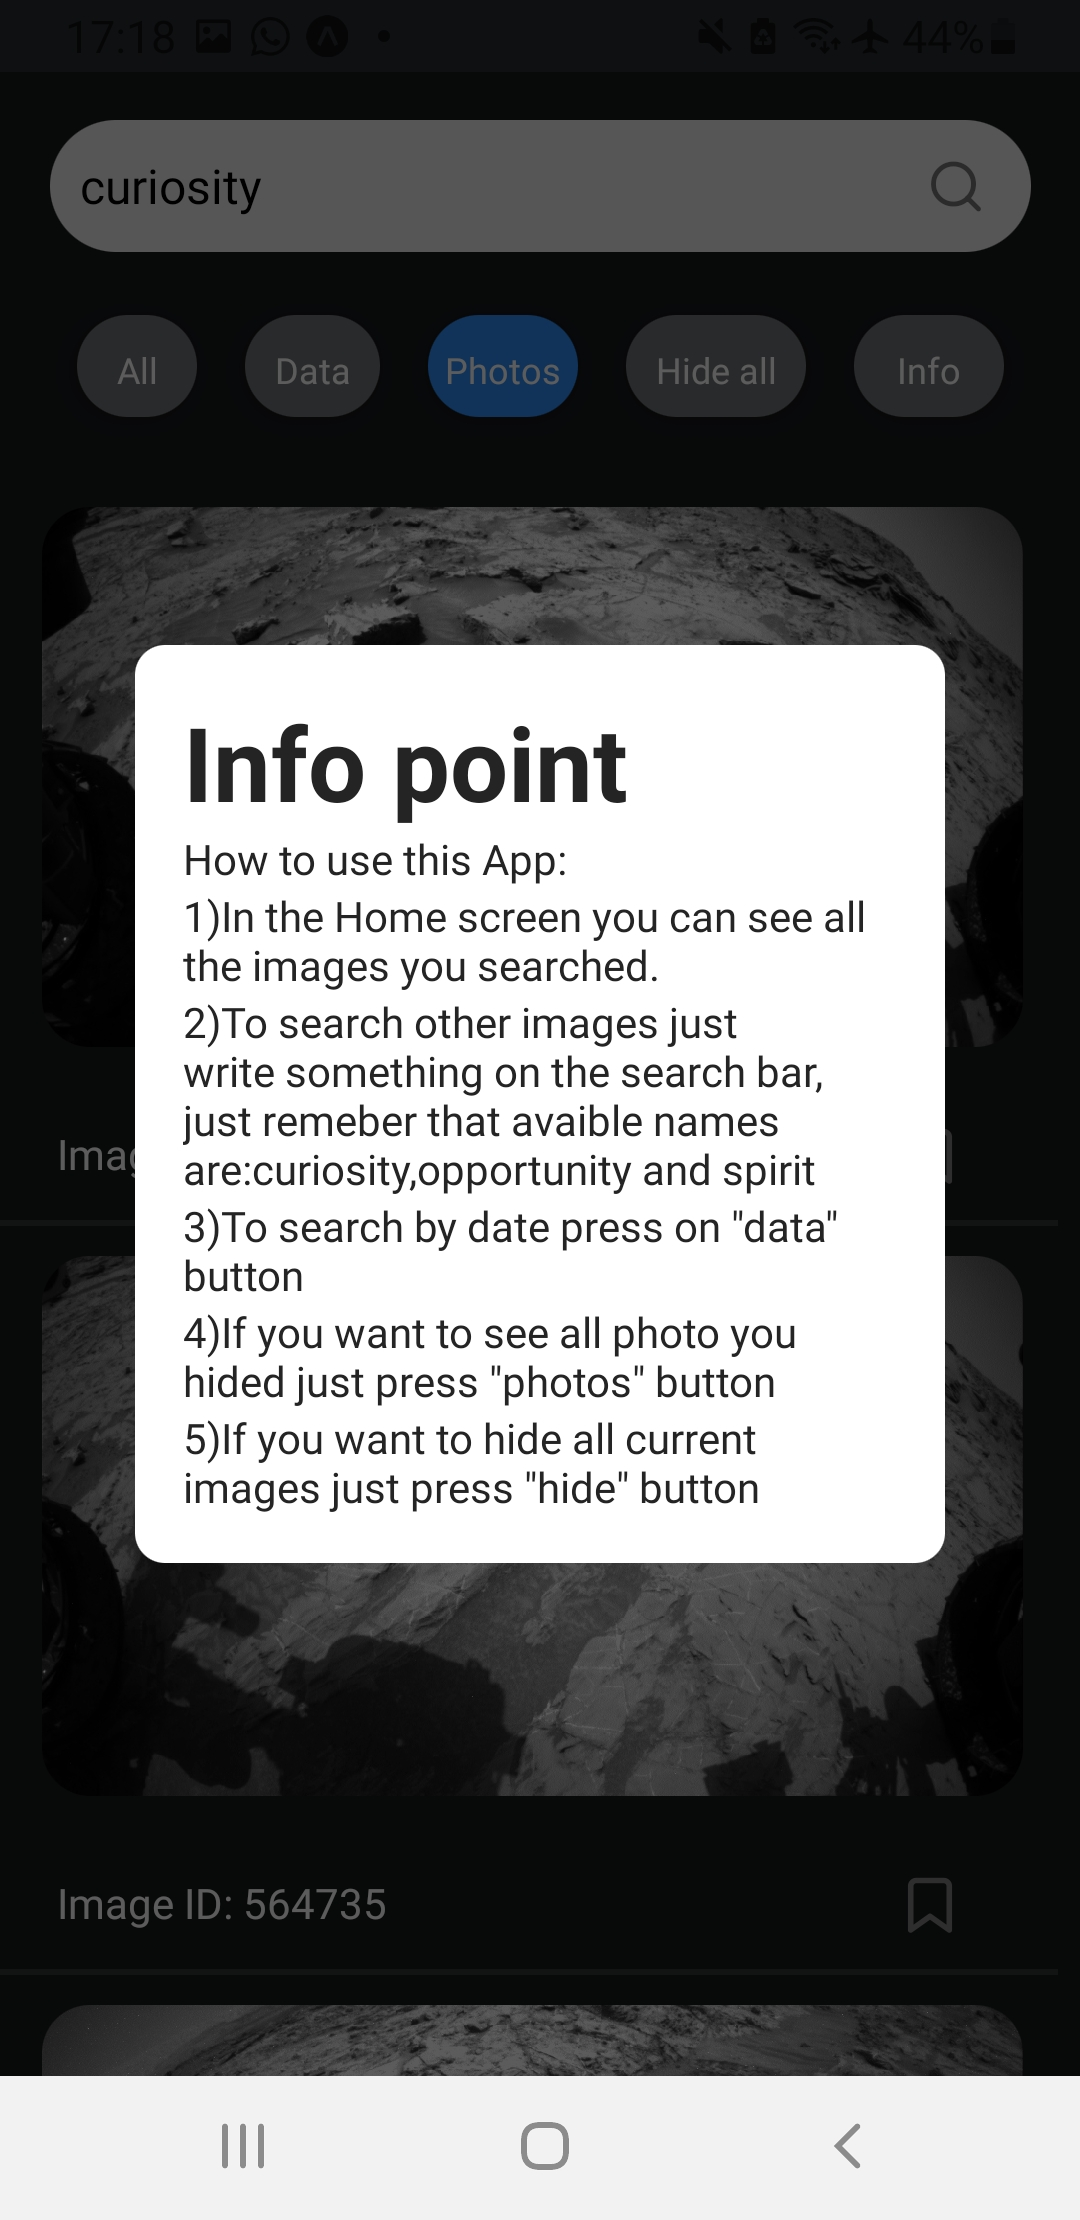
\includegraphics[width=5cm, height=10cm]{images/immaginiAndroid/infoPoint.jpg}
        \caption{\label{infoPointAndroid} Android info-point}
    \end{minipage}
    \hfill
    \begin{minipage}[h]{0.47\textwidth}
        \centering
        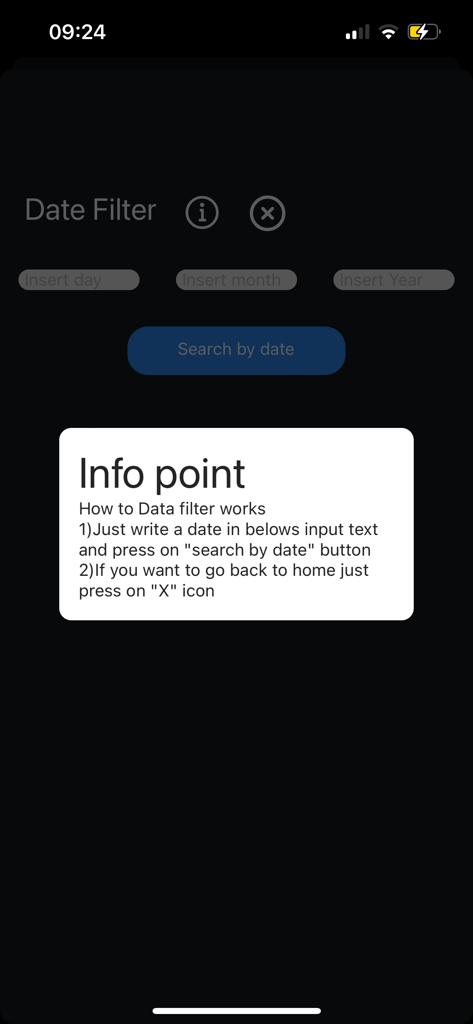
\includegraphics[width=5cm, height=10cm]{images/immaginiPhone/infoPoint.jpeg}
        \caption{\label{infoPointIphone} iPhone info-point}
    \end{minipage}
\end{figure}

\section{Procedura di Logout}
Per effettuare il logout dal proprio profilo, l'utente deve scorrere le immagini fino alla fine della lista e premere sul pulsante ``Log out". Una volta fatto ci\`o si viene reindirizzati alla schermata di \textit{sign in} o \textit{sign up}.

Nelle Fig 4.23 e 4.24 si pu\`o vedere che in Android si ha una migliore User Experience, in quanto il pulsante di logout non si soprappone ad altri componenti nativi del dispositivo: ad esempio sull'iPhone la barra orizzontale in fondo allo schermo si sovrappone al pulsante di Log out
\begin{figure}[H]
    \begin{minipage}[h]{0.47\textwidth}
        \centering
        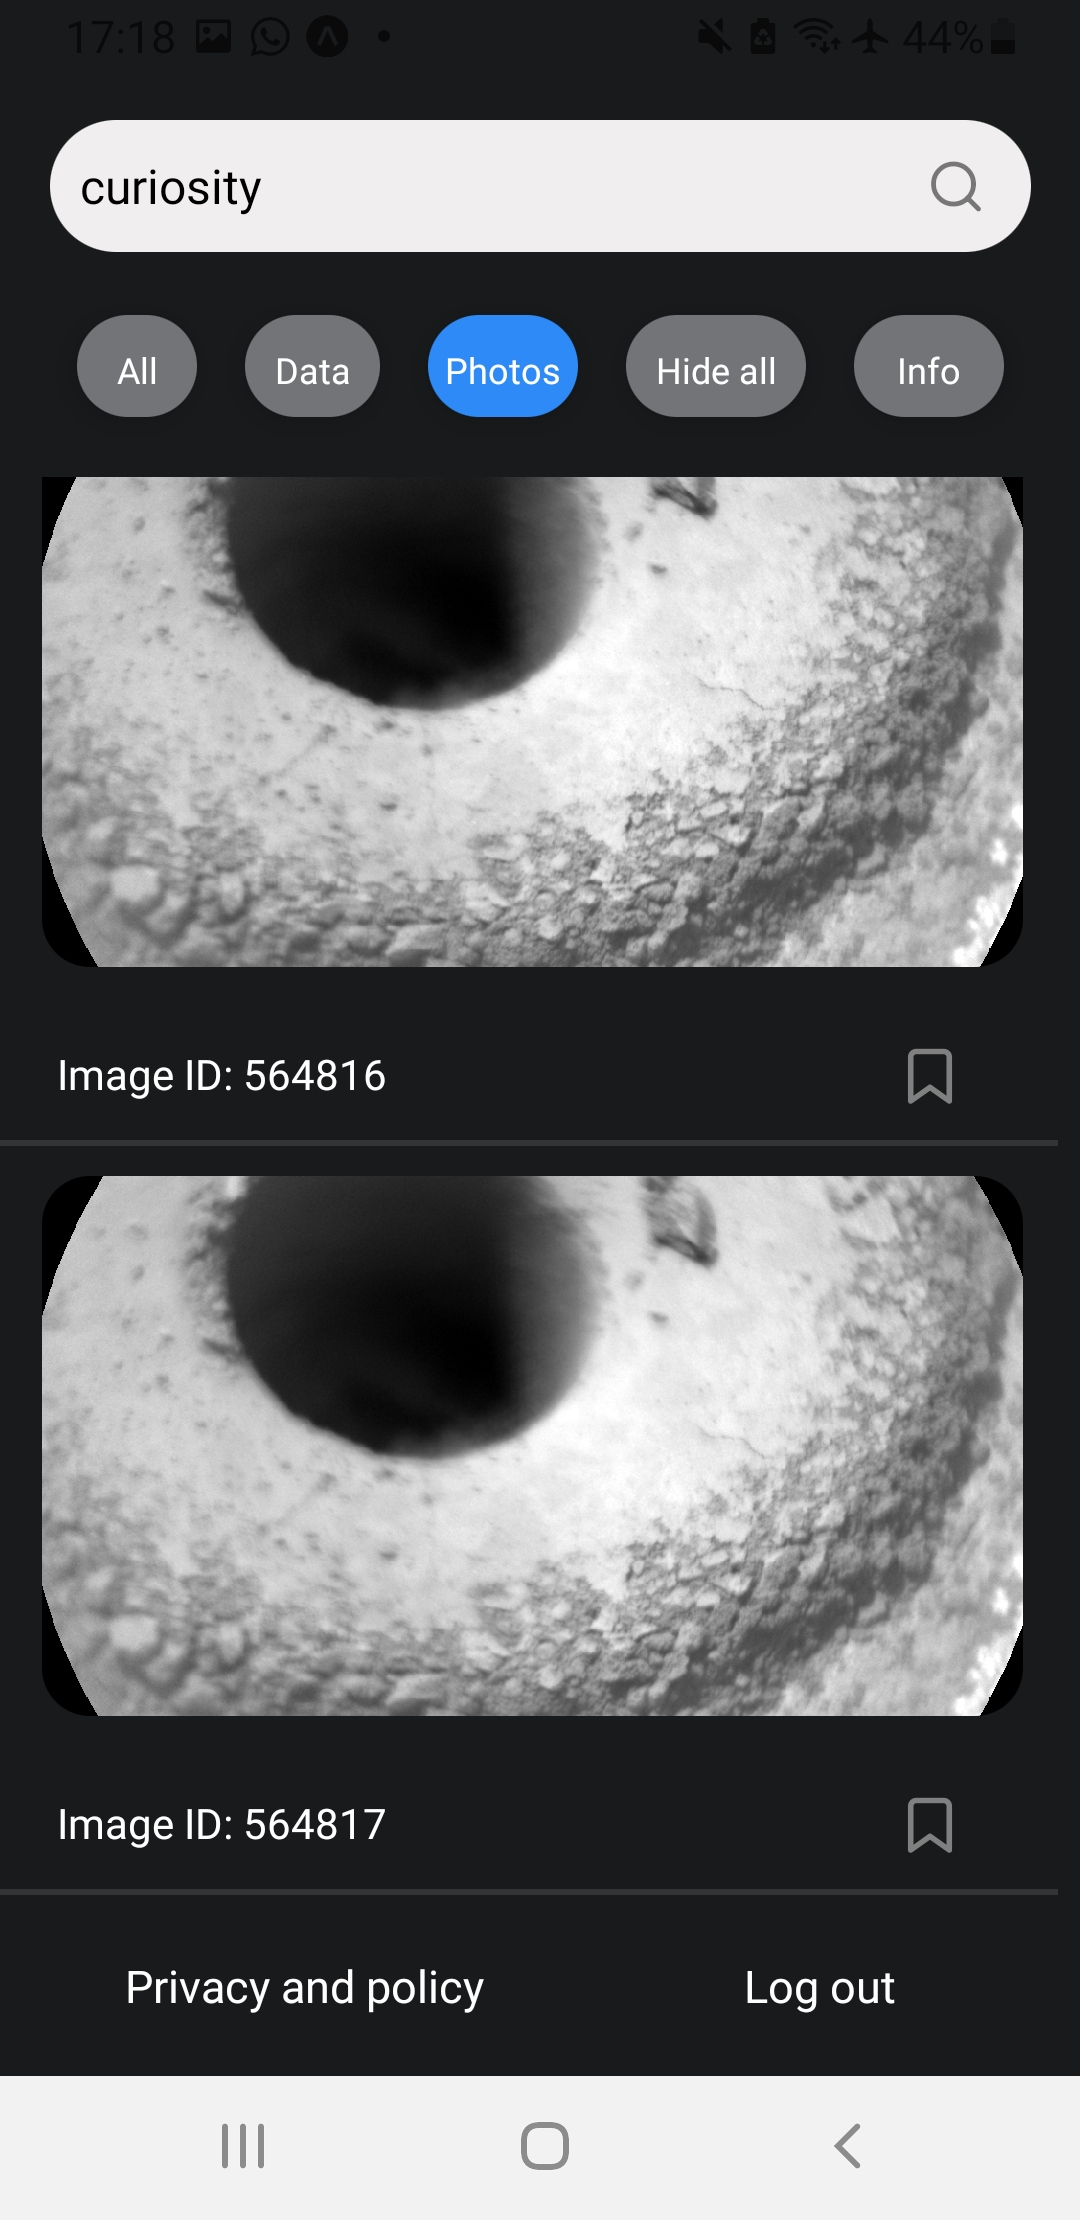
\includegraphics[width=5cm, height=10cm]{images/immaginiAndroid/logout.jpg}
        \caption{\label{logoutAndroid} Android pulsante di logout}
    \end{minipage}
    \hfill
    \begin{minipage}[h]{0.47\textwidth}
        \centering
        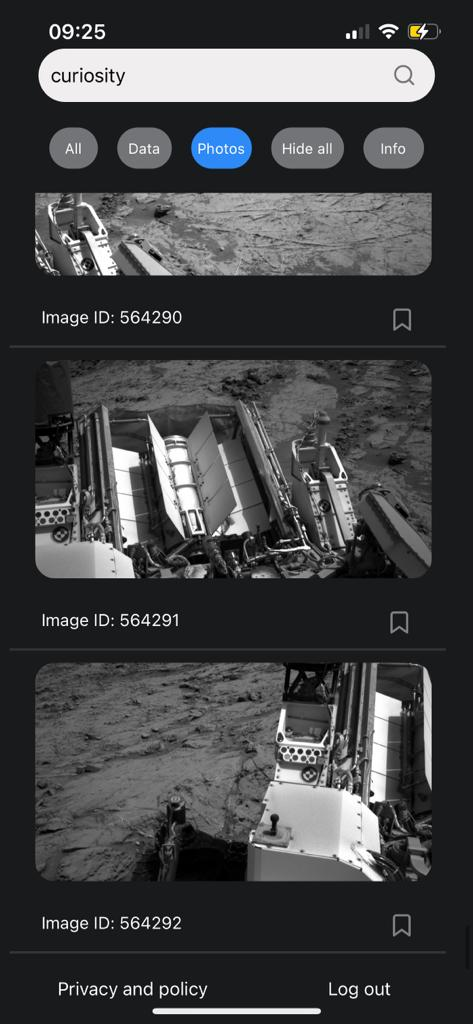
\includegraphics[width=5cm, height=10cm]{images/immaginiPhone/logout.jpeg}
        \caption{\label{logoutIphone} iPhone pulsante di logout}
    \end{minipage}
\end{figure}
